% ============================================================================
% ch3-results.tex — Chapter III: Results
% V4: sequential exhibits, enriched Discussion, Amundi reference
% ============================================================================
\chapterpage{Chapter\kern0.25em III}{Results}{images/IM3.jpeg}
\thispagestyle{chapterstart}

\vspace{2mm}


% ==============================================================================
% BEFORE THE TRANSMISSION MECHANISM — IMPACT LEAD-IN + EXHIBIT 10
% ==============================================================================

{\color{SEGreen}\textbf{\Large The repricing is already here}}
\vspace{1mm}

\noindent ClimVaR does not describe a distant tail risk. It reveals a present mispricing of digital infrastructure value under climate-naive assumptions. Unless otherwise specified, all results throughout this paper are reported under the BAU/MEAN pathway (RCP~8.5, business-as-usual transition policy, mean climate projection).

\vspace{2mm}

\exhibitcaption{10}{Panoramic results: ClimVaR across asset classes, AI scenarios, and adaptation strategies (BAU/MEAN).}

\begin{center}
\datatablesetup
\begin{tabularx}{\textwidth}{>{\raggedright\arraybackslash}p{3.5cm} >{\raggedleft\arraybackslash}X >{\raggedleft\arraybackslash}X >{\raggedleft\arraybackslash}X >{\raggedleft\arraybackslash}X >{\raggedleft\arraybackslash}X}
\toprule
\datatableheader
\thd{Portfolio} & \thd{V$_0$ (\$B)} & \thd{Baseline} & \thd{Selective} & \thd{Proactive} & \thd{Max red.} \\
\midrule
\textbf{Installed base} & \textbf{1,012} & \textbf{388} (38\%) & \textbf{305} (30\%) & \textbf{238} (24\%) & \textbf{39\%} \\
\quad United States & 393 & 108 (28\%) & 89 (23\%) & 72 (18\%) & 33\% \\
\quad Europe & 201 & 107 (53\%) & 81 (40\%) & 60 (30\%) & 44\% \\
\quad China & 198 & 111 (56\%) & 86 (44\%) & 67 (34\%) & 40\% \\
\quad APMEA\footnote{Asia-Pacific, Middle East, and Africa.} & 220 & 62 (28\%) & 49 (22\%) & 39 (18\%) & 37\% \\
\midrule
\textbf{Installed + LTG} & \textbf{1,992} & \textbf{1,008} (51\%) & \textbf{821} (41\%) & \textbf{669} (34\%) & \textbf{34\%} \\
\textbf{Installed + SAI} & \textbf{2,849} & \textbf{1,669} (59\%) & \textbf{1,366} (48\%) & \textbf{1,134} (40\%) & \textbf{32\%} \\
\textbf{Installed + AWB} & \textbf{5,590} & \textbf{3,671} (66\%) & \textbf{3,006} (54\%) & \textbf{2,536} (45\%) & \textbf{31\%} \\
\bottomrule
\end{tabularx}
\datatableclear
\end{center}

\exhibitsource{ClimVaR\% in parentheses = ClimVaR as \% of V$_0$. Max reduction = (Baseline $-$ Proactive) / Baseline. Under NZT, installed base ClimVaR rises to \$845B (83\%), with Proactive reducing it by 52\%.}

\begin{twocolbody}

{\color{SEGreen}\textbf{Aggregate mispricing at portfolio scale}}

\vspace{1mm}

\noindent The installed base of 8{,}572 data centers carries \textbf{\$388 billion} in climate-related value at risk---38.3\% of enterprise value under the BAU pathway. With prospective AI infrastructure, exposure rises to \textbf{\$1.0--3.7 trillion}, depending on the growth scenario. Even the most conservative pathway exceeds \$1 trillion. To put this in perspective: the installed-base figure alone is larger than the annual revenue of every listed data center operator combined.

This is why ClimVaR should be read as a measure of systematic mispricing. A traditional DCF assumes that cooling costs, carbon prices, outages, and physical damages remain within the historical range embedded in past cash flows. Climate-adjusted DCF removes that assumption. The 38.3\% gap is therefore not a tail event; it is the median repricing implied by the BAU/MEAN pathway.

\vspace{2mm}

{\color{SEGreen}\textbf{Intensity rises with AI scale}}

\vspace{1mm}

\noindent Exposure is not evenly distributed. Europe and China reach 53--56\% ClimVaR intensity, while the United States stands at 28\%---a twofold gap that reflects not just geography, but different channel structures. Business interruption dominates in the United States, carbon in Europe, and physical damage in Asia-Pacific. A single global reading of ``data center climate risk'' therefore obscures the real levers of action.

Just as importantly, \textbf{risk intensity increases with AI scale}. Installed-base intensity is 38\%; with AI infrastructure, it rises to 51\% (LTG), 59\% (SAI), and 66\% (AWB). This is not a simple scaling effect. It reflects a deeper shift in portfolio composition, where physical exposure becomes increasingly dominant as compute expands.

\end{twocolbody}

% ---- Transmission mechanism ----
\vspace{2mm}

\subsection*{The Transmission Mechanism}
\sectionsubtitle{How hazards propagate through risk channels to erode enterprise value}
\greensep

\exhibitcaption{11}{The transmission map: hazards to enterprise value loss.}
\begin{center}
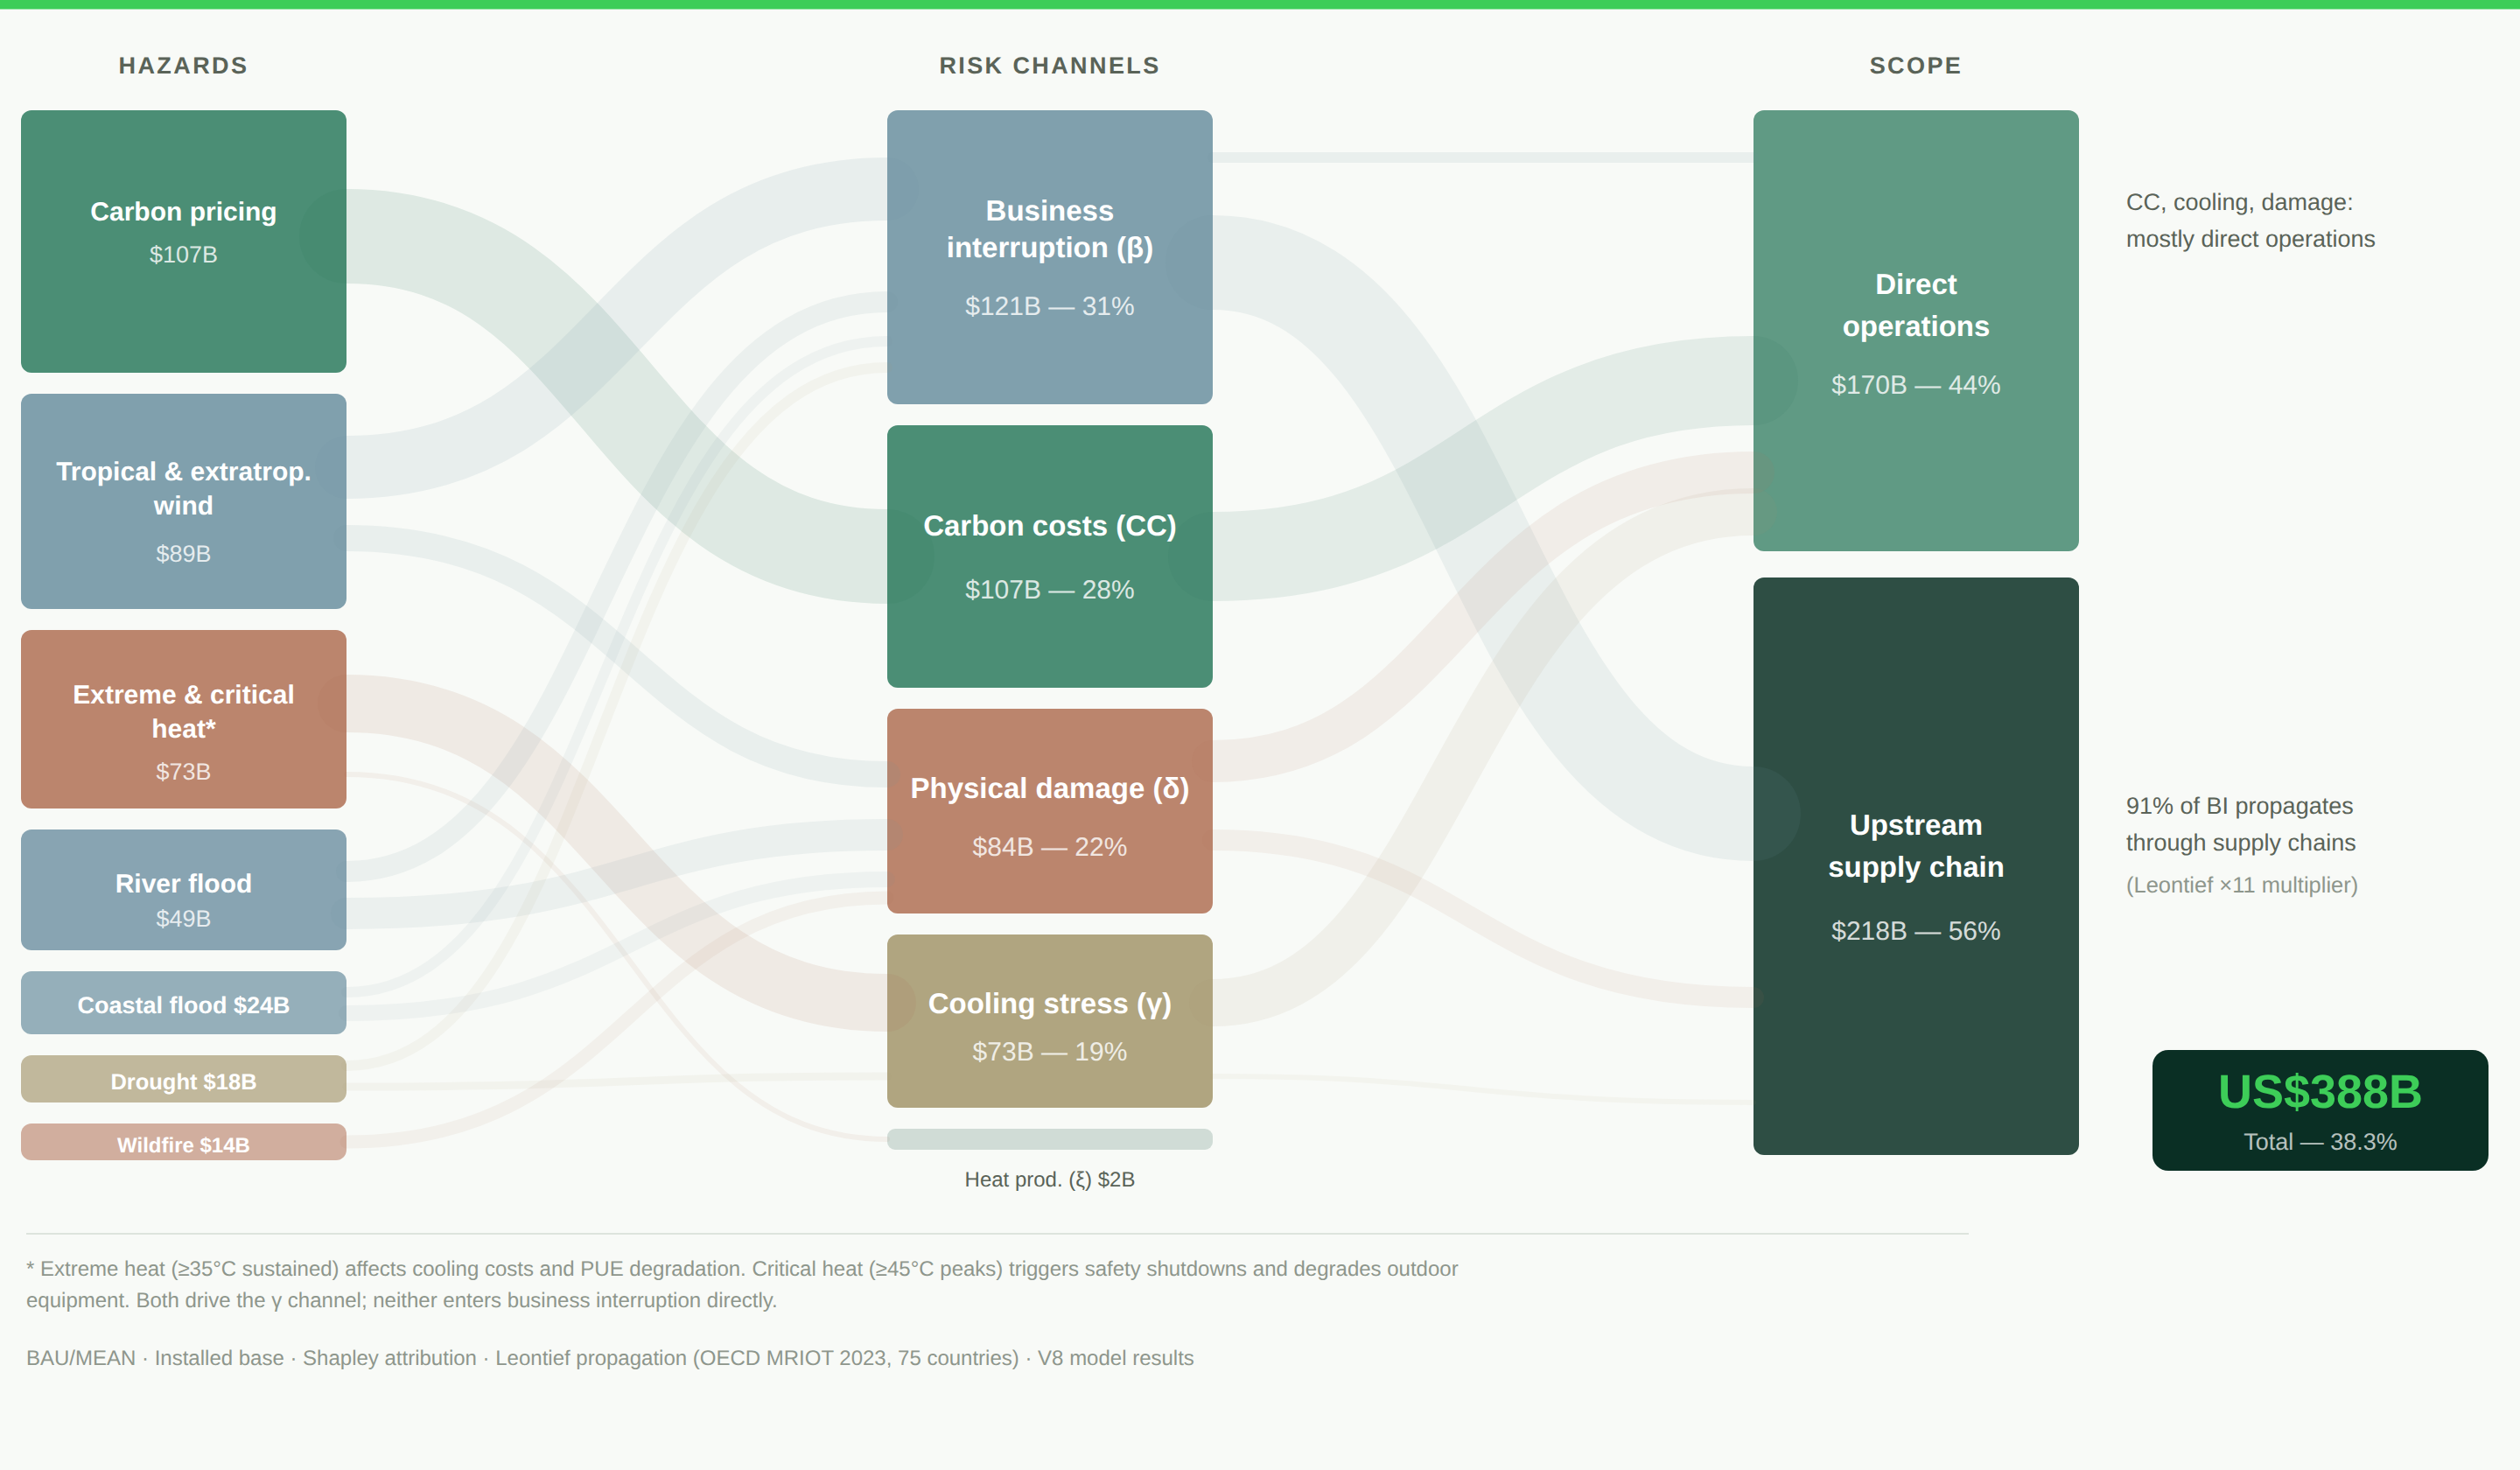
\includegraphics[width=\textwidth]{images/exhibit11_sankey.png}
\end{center}
\exhibitsource{Seven hazards propagate through four principal risk channels to erode enterprise value. Ribbon width proportional to US\$ value. Shapley attribution for hazard-to-channel mapping. BAU/MEAN, installed base.}

\begin{twocolbody}

{\color{SEGreen}\textbf{From hazards to financial channels}}

\vspace{1mm}

\noindent Exhibit~11 makes visible the mechanism that the aggregate figure of \$388~billion tends to obscure. Climate risk does not arrive at the balance sheet in the abstract. It passes through a sequence: hazards strike physical systems, physical systems disrupt operations, and those disruptions are translated into discounted cash-flow losses. What the transmission map shows is therefore not an illustration but the architecture of the loss itself.

On the left, seven hazards are ranked by contribution. Tropical wind dominates, followed by extreme heat and river flood, while carbon pricing appears as a transition hazard with a weight comparable to the largest physical drivers. This ordering is already instructive. A naive reading of data-center exposure might expect flood to dominate, because flood is the most visible and the most intuitively destructive hazard. Yet tropical wind ranks first because its effects travel further: not only through direct site exposure, but through semiconductor fabrication, electrical equipment manufacturing, logistics corridors, and other supply-chain dependencies whose disruption propagates across the portfolio.

\vspace{5mm}

{\color{SEGreen}\textbf{Why the map changes the diagnosis}}

\vspace{1mm}

\noindent On the right, hazards are aggregated into risk channels. Business interruption is the largest channel, ahead of carbon costs, physical damages, and cooling penalties. This matters because the ranking of channels is not the ranking of hazards: a single hazard can contribute to several channels simultaneously, and a single channel can be fed by several hazards at once. Tropical wind, for instance, contributes both to business interruption and to physical damage; extreme heat drives cooling stress through rising ambient temperatures. The map therefore formalizes the non-additivity of climate risk.

This is also why Shapley decomposition is essential to the framework. Without it, one would either double-count the contribution of a hazard that affects several channels, or collapse distinct mechanisms into a single undifferentiated estimate---both analytically fatal for adaptation planning. The model does not merely say that climate risk is large; it shows how it is transmitted, through which levers it becomes financially material, and therefore where adaptation can act with the greatest force.

\end{twocolbody}

% ==============================================================================
% FINDING 1 — PAGE 1 of 2
% ==============================================================================
\clearpage\thispagestyle{chapterstart}

{\color{SEGreen}\subsection*{Finding 1: Unpriced Exposure}}
\sectionsubtitle{Climate risk erodes 38\% of current data center asset value}
\greensep

\begin{twocolbody}

{\color{SEGreen}\textbf{ClimVaR as structural repricing of the asset}}

\vspace{1mm}

\noindent The installed base of 8{,}572 data centers, valued at US\$1{,}012~billion under standard discounted cash-flow assumptions, carries US\$388~billion in climate-adjusted value erosion---38.3\% of enterprise value. No current valuation framework captures this figure, no disclosure regime requires its reporting, no insurance product prices it. US\$388B exceeds the combined annual revenue of every publicly listed data center operator. It is a lower bound.

ClimVaR can be interpreted in the same way as a credit impairment or a permanent margin compression: not as the probability of a catastrophic event, but as a structural repricing of the asset over its 15--25 year lifetime. A facility with a climate-naive valuation of US\$100~million and a ClimVaR of 38\% does not face a 38\% chance of total loss; it faces a future in which, on the median pathway, cooling penalties, carbon costs, outages, and damage combine to erode US\$38~million of its discounted cash flows.

\vspace{5mm}

{\color{SEGreen}\textbf{Five channels, three central observations}}

\vspace{1mm}

\noindent The aggregate figure combines five risk channels, each operating through a distinct financial mechanism and each responding to different adaptation levers. Three observations structure the decomposition that Exhibit~12 presents. First, business interruption leads at 31\% of total ClimVaR, but 91\% of it propagates through supply chains rather than through direct facility disruption---a ratio of eleven to one between indirect and direct exposure. An operator monitoring only on-site hazards misses the primary risk vector. Second, carbon costs represent 28\% and span all three scopes, but are almost entirely Scope~2 (location-based): US\$106B of US\$107B originate in grid carbon intensity, not in on-site emissions. Scope~3 is included in the model but negligible at this scale. The PPA\footnote{Power Purchase Agreement: a long-term contract to buy electricity directly from a renewable energy producer, bypassing grid carbon exposure.} is therefore the primary lever for transition risk. Third, the physical channels---business interruption, damages, cooling---together account for 72\% of total ClimVaR on the installed base; carbon accounts for 28\%. This ratio inverts when AI infrastructure enters the portfolio, as Finding~3 documents.

From an investment perspective, the distinction between channels matters more than the aggregate number. A credit analyst can treat ClimVaR as an additional spread over the climate-naive discount rate, but an engineer or operator needs to know whether that spread comes from outage risk, from cooling penalties, from structural damage, or from carbon. The same dollar of adaptation budget does not buy the same reduction in each channel. Exhibit~12 is therefore not a purely descriptive breakdown; it is the bridge between the macro figure (US\$388B) and the micro-level levers that later sections quantify.

\end{twocolbody}

\vspace{2mm}
\exhibitcaption{12}{ClimVaR decomposition by risk channel---installed base, BAU/MEAN.}

\begin{center}
\datatablesetup
\begin{tabularx}{\textwidth}{>{\raggedright\arraybackslash}p{3.8cm} >{\raggedleft\arraybackslash}p{1.4cm} >{\raggedleft\arraybackslash}p{1cm} >{\raggedright\arraybackslash}X}
\toprule
\datatableheader
\thd{Risk Channel} & \thd{\$B} & \thd{Share} & \thd{Mechanism} \\
\midrule
Business interruption ($\beta$) & 121.4 & 31\% & Extreme events, grid stress, downtime \\
Carbon costs (CC$^{1,2,3}$) & 107.1 & 28\% & Grid emissions $\times$ carbon price \\
Physical damages ($\delta$) & 84.1 & 22\% & Floods, storms, structural damage \\
Cooling penalty ($\gamma$) & 72.6 & 19\% & Ambient temperature $\to$ energy cost \\
Heat productivity ($\xi$) & 2.4 & 1\% & Worker/equipment efficiency loss \\
\midrule
\textbf{Total ClimVaR} & \textbf{387.5} & \textbf{100\%} & \\
\bottomrule
\end{tabularx}
\datatableclear
\end{center}

\begin{twocolbody}

{\color{SEGreen}\textbf{Tropical wind versus flood: severity and reach}}

\vspace{1mm}

\noindent Why does tropical wind rank first among hazards, ahead of flood? The answer lies in the distinction between severity and reach. River flood inflicts catastrophic damage at exposed sites but affects only facilities in floodplains. Tropical wind propagates through supply chains serving the entire portfolio: a typhoon disrupting semiconductor fabrication in Taiwan degrades every facility depending on those inputs, regardless of location. At portfolio level, a hazard touching many facilities indirectly outweighs one devastating a few directly. The Sankey in Exhibit~11 makes this visible: the tropical-wind ribbon is wide because its consequences travel further through the network.

\vspace{3mm}

{\color{SEGreen}\textbf{What \$388B does not capture}}

\vspace{1mm}

\noindent The framework does not capture nature-related risk---water stress, biodiversity constraints, ecosystem degradation around cooling sources---nor systemic externalities: grid strain from concentrated AI load, community displacement, or cascading service interruptions across interconnected facilities. Each omitted channel would widen, not narrow, the exposure estimate. The \$388B figure is therefore the floor of an exposure range whose ceiling remains unquantified. For investors and regulators: climate risk on digital infrastructure is already material at the lower bound; model refinements are more likely to move the estimate upward than downward.

\end{twocolbody}


% ==============================================================================
% FINDING 1 — PAGE 2 of 2
% ==============================================================================
\clearpage\thispagestyle{chapterstart}

{\color{SEGreen}\subsection*{Finding 1: Unpriced Exposure}}
\sectionsubtitle{Four regions, five channels, and the geography of \$388 billion}
\greensep

\exhibitcaption{13}{US\$388 billion decomposed: four regions, five channels, one treemap.}
\begin{center}
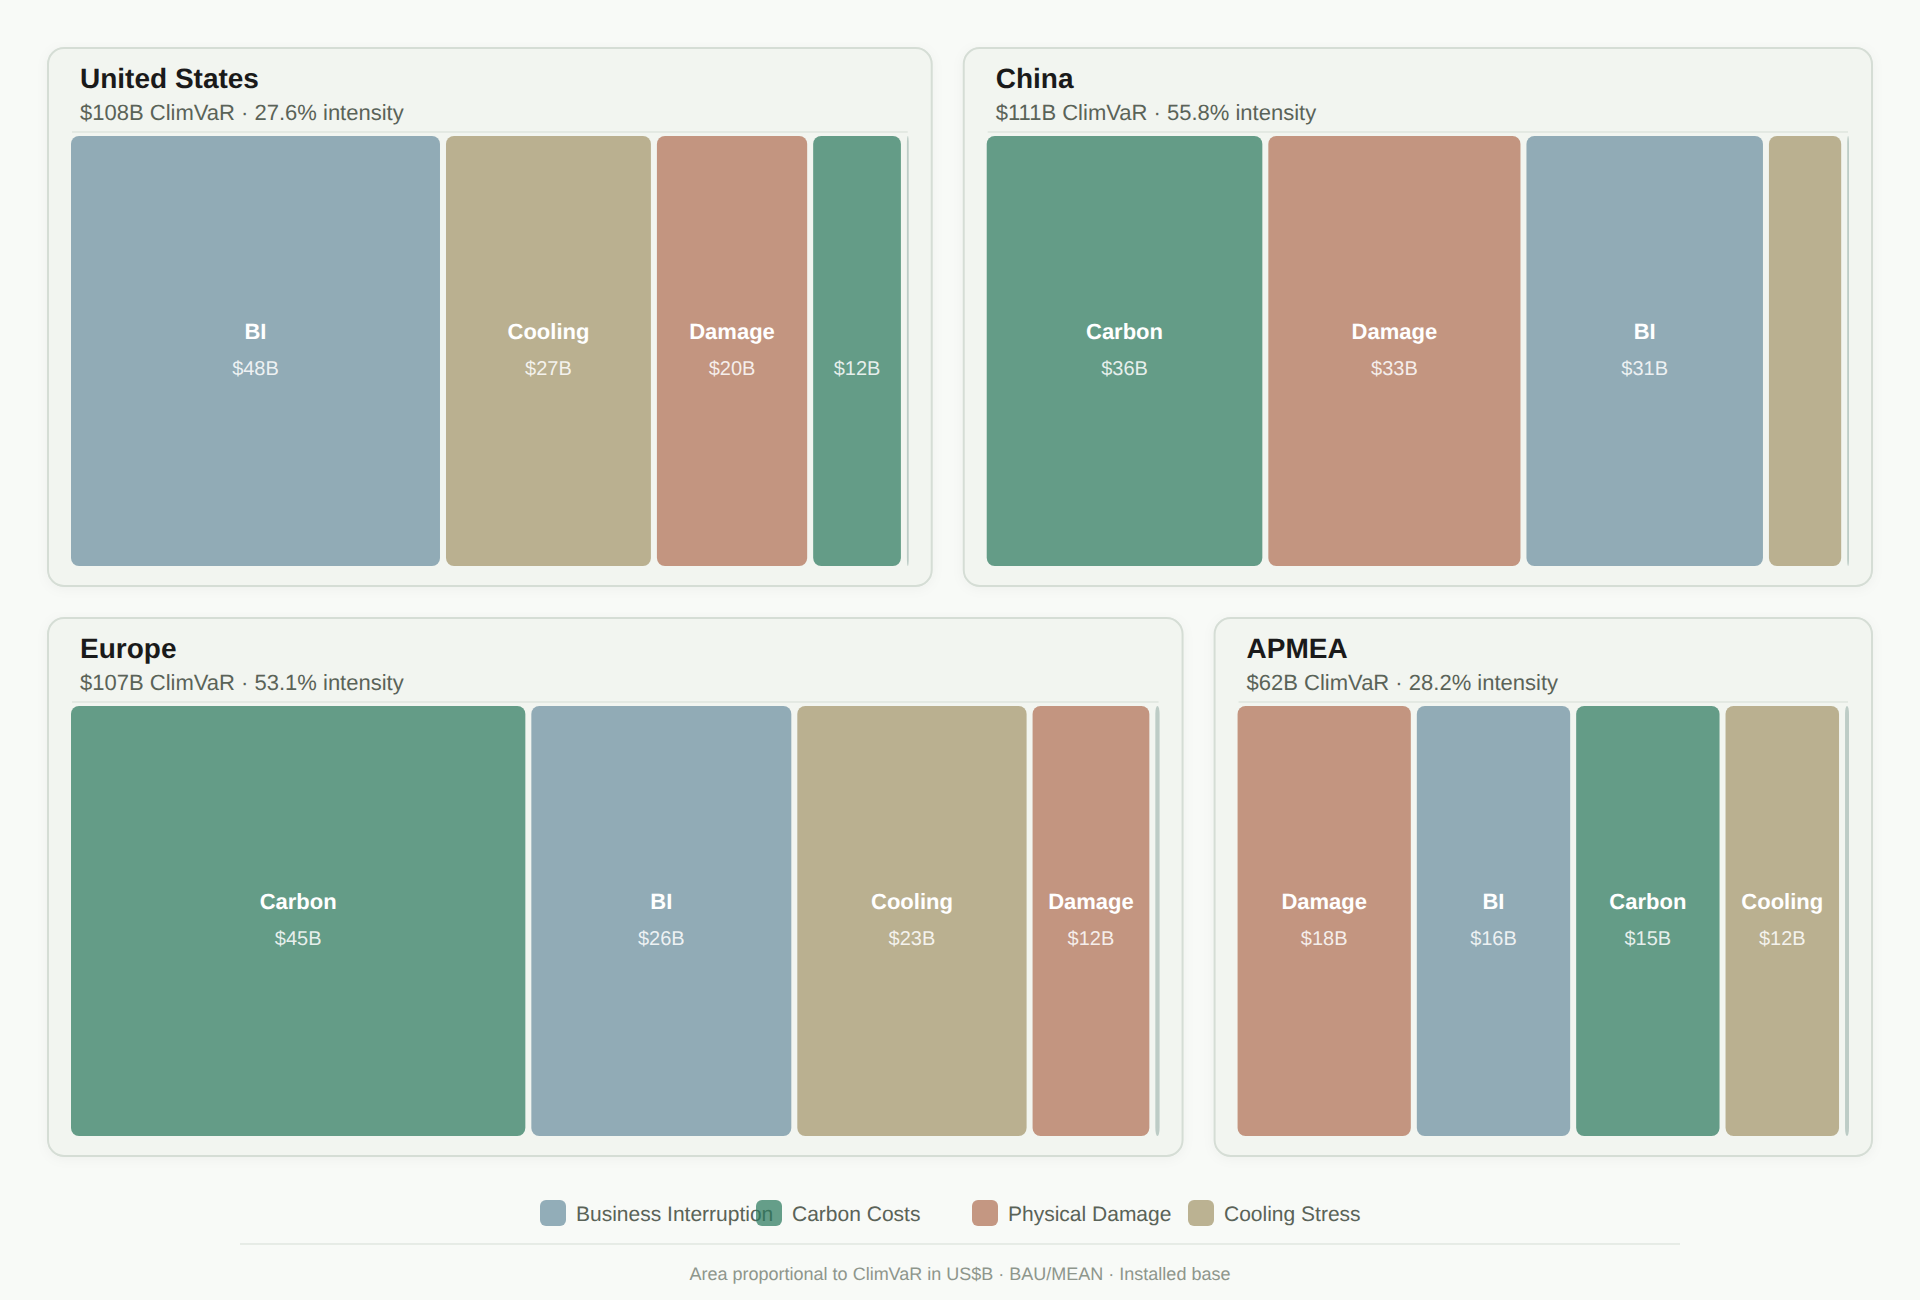
\includegraphics[width=\textwidth]{images/exhibit13_treemap.png}
\end{center}
\exhibitsource{Area proportional to ClimVaR in US\$B. Outer rectangles = regions; inner tiles = risk channels. BAU/MEAN, installed base. The dominant tile in each region identifies the primary adaptation lever.}

\begin{twocolbody}
{\color{SEGreen}\textbf{One map, two dimensions of exposure}}

\vspace{1mm}

\noindent The treemap encodes the same US\$388B from two angles simultaneously: region and channel. The area of each tile is proportional to dollar exposure, so that a single glance shows three things: where the money is, which channel drives it, and how the composition shifts by geography. Outer rectangles show regions; inner tiles show the five risk channels. The dominant tile in each region is therefore the first-order adaptation lever. Note that business interruption (91\% supply-chain-driven) and carbon costs (99\% Scope~2) are both quasi-exclusively upstream exposures: the treemap therefore also maps supply chain vulnerability, even though it is organized by financial channel.

\vspace{5mm}

{\color{SEGreen}\textbf{Four fingerprints, four risk structures}}

\vspace{1mm}

\noindent The United States concentrates 28\% of global exposure---US\$108B---but at the lowest intensity (27.6\%). Business interruption fills nearly half the US rectangle, a consequence of dependence on East Asian semiconductor supply chains and grid stress during extreme heat events. Europe shows a different signature: US\$45B in carbon costs alone, driven by higher carbon pricing under the EU~ETS\footnote{European Union Emissions Trading System: the world’s largest carbon market, covering approximately 40\% of EU greenhouse gas emissions.} and residual grid emission intensity. China carries a triple threat of comparable magnitude---carbon (US\$36B), physical damage (US\$33B), and business interruption (US\$31B)---so that intervention on any single channel leaves roughly two-thirds of the exposure intact. APMEA is the smallest rectangle but the most evenly distributed across channels, a profile that resists single-lever intervention.

\vspace{5mm}

\noindent The asymmetry between these four fingerprints is the diagnostic: the US\$388B headline is not a single problem but a family of regional problems that share a magnitude and differ in mechanism. A uniform adaptation strategy systematically underinvests in the dominant channel. The Shapley decomposition quantifies this fingerprint from the global portfolio down to individual facilities.

\end{twocolbody}

% ==============================================================================
% FINDING 2 — GEOGRAPHIC DISPERSION OF RISK AND ADAPTATION VALUE
% ==============================================================================

\vspace{6mm}

\subsection*{Finding 2: Geography changes the diagnosis}
\sectionsubtitle{Unevenly distributed, differently composed}
\greensep

\begin{twocolbody}

{\color{SEGreen}\textbf{The same asset class, four different risk worlds}}

\vspace{1mm}

\noindent The global headline conceals a decisive fact: there is no single geography of data-center climate risk. The installed base spans 8{,}572 facilities across four major regions, but the exposure profile is not merely a matter of different magnitudes; it is a matter of different structures. Europe and China reach ClimVaR intensities of 53--56\%, while the United States stands at 28\%. That twofold spread cannot be explained by hazard maps alone. It reflects the interaction between regional climate conditions, electricity systems, industrial dependencies, and carbon-policy regimes.

This distinction matters because adaptation is not purchased against ``climate risk'' in the abstract. It is purchased against specific transmission mechanisms. A portfolio exposed primarily through business interruption requires different interventions from one exposed primarily through carbon, cooling, or direct damage. Once risk is decomposed by geography and channel, the idea of a universal adaptation playbook begins to collapse.

\vspace{5mm}

{\color{SEGreen}\textbf{Regional intensity is only the first layer of the problem}}

\vspace{1mm}

\noindent The first reading of the evidence is intuitive: some regions are simply riskier than others. But this is only the first layer. The deeper point is that regional risk intensity and regional risk composition do not move together in a simple way. The United States carries the largest absolute share of enterprise value and a large share of total ClimVaR, yet does so at lower relative intensity. Europe carries less enterprise value but much higher relative erosion because carbon pricing and grid exposure weigh more heavily on long-term cash flows. China combines high intensity with a more diversified set of channels, making it less responsive to narrow interventions.

In other words, a region can matter for three different reasons: because it is large, because it is intense, or because its internal composition makes adaptation harder. Those three logics do not always coincide. This is precisely why a portfolio-wide average is analytically weak: it merges scale, intensity, and composition into a single figure and thereby obscures the actual economics of intervention.

\vspace{5mm}

{\color{SEGreen}\textbf{Why a global average misallocates adaptation capital}}

\vspace{1mm}

\noindent A global average encourages the wrong instinct: spread adaptation capital evenly, or prioritize the largest regions first. Yet neither rule follows from the evidence. If one region is dominated by carbon exposure, another by business interruption, and a third by physical damages, then the same dollar does not buy the same protection in each geography. Capital allocation must therefore be differentiated not only by hazard level, but by the structure of loss transmission.

This is one of the central analytical contributions of the framework. The model does not stop at saying that geography matters; it specifies \textbf{how} it matters. It identifies where the portfolio is most eroded, through which channels that erosion occurs, and therefore where targeted adaptation is likely to produce the greatest reduction in value at risk. Geography is not a backdrop to the model. It is one of its principal explanatory dimensions.

\end{twocolbody}

\vspace{2mm}
\exhibitcaption{14}{Regional ClimVaR intensity and adaptation headroom across the installed base.}

\begin{center}
\datatablesetup
\begin{tabularx}{\textwidth}{>{\raggedright\arraybackslash}p{3.2cm} >{\raggedleft\arraybackslash}X >{\raggedleft\arraybackslash}X >{\raggedleft\arraybackslash}X >{\raggedleft\arraybackslash}X >{\raggedleft\arraybackslash}X}
\toprule
\datatableheader
\thd{Region} & \thd{V$_0$ (\$B)} & \thd{Baseline} & \thd{Selective} & \thd{Proactive} & \thd{Max red.} \\
\midrule
United States & 393 & 108 (28\%) & 89 (23\%) & 72 (18\%) & 33\% \\
Europe & 201 & 107 (53\%) & 81 (40\%) & 60 (30\%) & 44\% \\
China & 198 & 111 (56\%) & 86 (44\%) & 67 (34\%) & 40\% \\
APMEA\footnote{Asia-Pacific, Middle East, and Africa.} & 220 & 62 (28\%) & 49 (22\%) & 39 (18\%) & 37\% \\
\bottomrule
\end{tabularx}
\datatableclear
\end{center}

\begin{twocolbody}

{\color{SEGreen}\textbf{Adaptation value also varies by region}}

\vspace{1mm}

\noindent Exhibit~14 adds a second layer to the diagnosis: not only are regional risks uneven, but the value of adaptation is uneven as well. Europe shows the highest proportional reduction under the Proactive strategy, with a 44\% reduction from baseline. China follows at 40\%, then APMEA at 37\%, while the United States reaches 33\%. The implication is important: the most adaptation-responsive regions are not necessarily the largest, but they may offer the greatest risk reduction per unit of intervention.

This is where the model becomes operationally powerful. It makes visible not only where risk is located, but where adaptation has the strongest leverage over future value erosion. For a global operator, this is the difference between adaptation as generic resilience spending and adaptation as disciplined capital allocation.

\end{twocolbody}

% ==============================================================================
% FINDING 2 — PAGE 2
% ==============================================================================
\clearpage\thispagestyle{chapterstart}

\subsection*{Finding 2: Geography changes the diagnosis}
\sectionsubtitle{Why adaptation must be targeted, not standardized}
\greensep

\exhibitcaption{15}{Four fingerprints: regional channel composition as radar overlay.}
\begin{center}
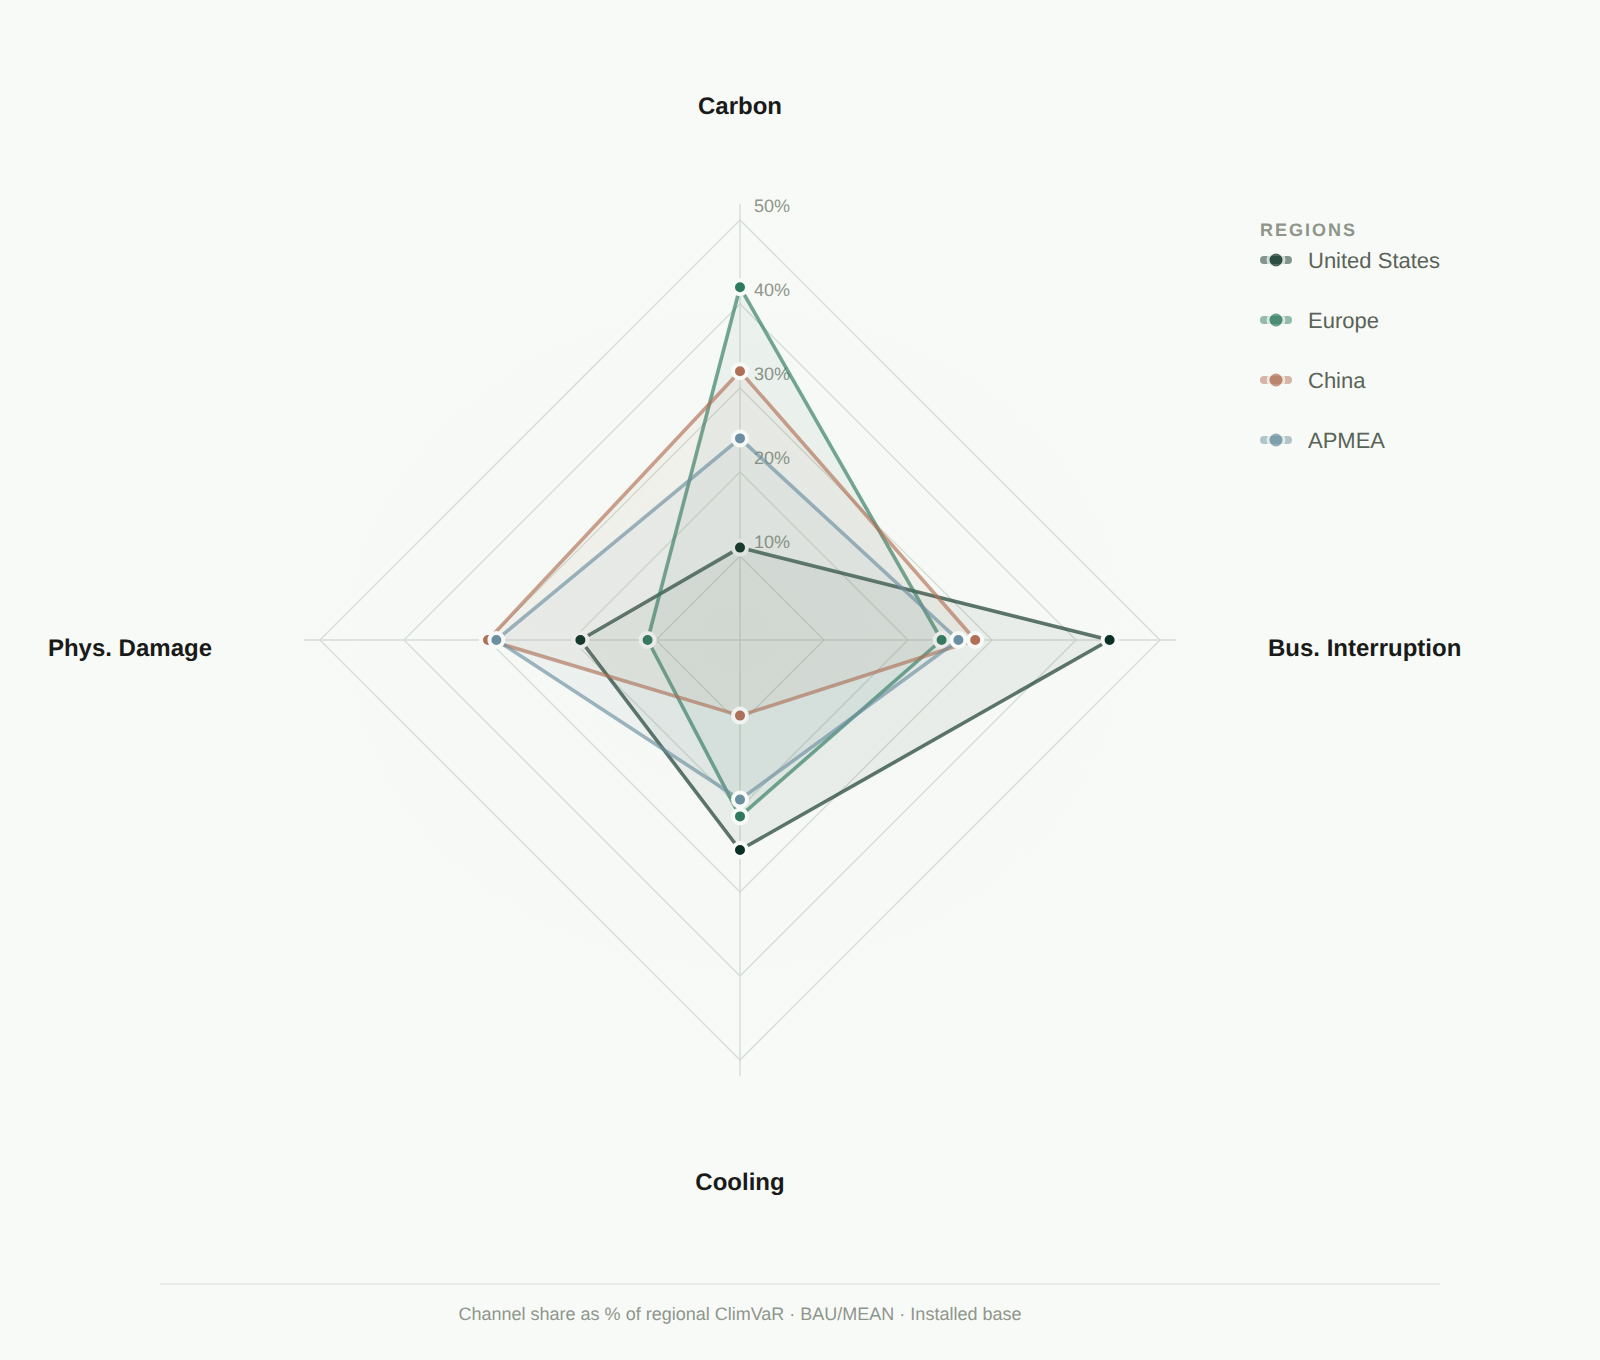
\includegraphics[width=0.72\textwidth]{images/exhibit15_radar.png}
\end{center}
\exhibitsource{Each polygon is one region's channel fingerprint, expressed as \% of regional ClimVaR. The asymmetry between shapes shows why a uniform adaptation strategy fails. BAU/MEAN, installed base.}

\begin{twocolbody}

{\color{SEGreen}\textbf{What the radar chart reveals}}

\vspace{1mm}

\noindent The radar shows what tables cannot: regions differ not only in \emph{how much} ClimVaR they carry, but in \emph{how they carry it}. Each geography has a distinct risk fingerprint. The United States is pulled outward by business interruption, Europe by carbon, China by a multi-channel structure, and APMEA by a flatter profile. These shapes matter because adaptation strategies act on shapes, not just on totals.

The table says that Europe is highly exposed and highly responsive to proactive adaptation; the radar explains why. Carbon dominates its risk architecture, and carbon is a channel where targeted interventions have strong effect. China, by contrast, shows no single dominant channel, so narrow measures have limited leverage unless they are combined.

\vspace{3mm}
{\color{SEGreen}\textbf{Four regions, four adaptation logics}}

\vspace{1mm}

\noindent The United States calls for a \emph{continuity} logic: with business interruption dominant, resilience hinges on supply-chain robustness, backup systems, and reduced downtime. Europe calls for a \emph{decarbonization-and-procurement} logic: carbon is central to value erosion, making power sourcing and grid exposure decisive. China calls for a \emph{portfolio} logic, since exposure is spread across several large channels. APMEA calls for a \emph{balancing} logic, as its more even profile resists single-lever intervention.

Regional fingerprints shift the question from ``Where is risk high?'' to ``What kind of intervention is economically rational here?'' They preserve analytical rigor while making visible the use value of the framework for capital planning, siting, resilience, and energy strategy.

\vspace{3mm}
{\color{SEGreen}\textbf{Geography determines what counts as adaptation}}

\vspace{1mm}

\noindent The strongest implication of Finding~2 is not just that regions should be ranked differently. It is that geography changes the meaning of adaptation. In one region, adaptation mainly means reducing outage risk; in another, lowering carbon exposure; in a third, managing physical damage and cooling stress together. Treating all of these under a single adaptation label is conceptually convenient but economically misleading.

The framework matters beyond the headline estimate because it offers a white-box view of regional heterogeneity---transparent, decomposable, and usable for scenario design. It shows what black-box risk scores often miss: adaptation is not simply a volume of spend, but a geography-specific strategy whose effectiveness depends on \textbf{matching interventions to the regional structure of loss}.

\end{twocolbody}

% ==============================================================================
% FINDING 3 — PAGE 1 of 2
% From geography to amplification: AI makes it worse
% ==============================================================================

\clearpage\thispagestyle{chapterstart}

\subsection*{Finding 3: AI Amplification}
\sectionsubtitle{AI-era infrastructure carries $\times$2.6 the physical risk per GW}
\greensep

\begin{twocolbody}

{\color{SEGreen}\textbf{From carbon-driven to physically-driven risk}}

\vspace{1mm}

\noindent The AI build-out does not replicate the risk profile of the installed base---it inverts it. On legacy facilities, carbon costs represent 28\% of total ClimVaR and physical channels 72\%. On AI-era facilities, physical channels account for 93--94\% while carbon drops to 6--7\%. The inversion is not gradual: even the most conservative growth scenario (Limits to Growth, adding 63~GW) pushes the physical share above 93\%. 

This has a direct consequence that no sustainability strategy focused on renewable procurement can resolve. Net-zero commitments address the carbon component---which on AI infrastructure represents less than one-tenth of the exposure. For operators who have built their climate strategy around Scope~2 reductions, the centre of gravity of risk has moved somewhere their existing toolkit barely touches.

\vspace{5mm}

{\color{SEGreen}\textbf{A portfolio that adds capacity and multiplies physical exposure}}

\vspace{1mm}

\noindent From the installed base (90.8~GW) to the Abundance Without Boundaries portfolio (386~GW), capacity grows by a factor of 4.3. Physical risk grows by a factor of 11---which yields an amplification of $\times$2.6 per GW added. Three mechanisms drive this non-linearity.

First, \textit{geographic concentration}: AI facilities cluster in regions combining cheap power with fast permitting---the US South, the US East Coast, parts of China and Southeast Asia---the same regions with elevated physical climate exposure. The installed base is geographically diverse; AI additions concentrate risk. Second, \textit{power density}: AI racks at 30--100+~kW generate more waste heat per square meter, so that a cooling system failure at a 5~kW/rack legacy facility is an inconvenience, while at a 60~kW/rack AI cluster it triggers thermal shutdown within minutes. Third, \textit{supply chain criticality}: AI training runs are non-interruptible workloads where a single disruption can invalidate weeks of compute, creating losses that far exceed the downtime itself.

Under the Abundance Without Boundaries scenario, several regional portfolios approach conditions where ClimVaR exceeds V$_0$---that is, where climate-adjusted residual value approaches zero or turns negative under tail conditions. Europe reaches 93.5\% ClimVaR intensity; China 79.5\%; the United States 64.3\%. Only APMEA, at 33.5\%, remains in moderate territory. The channels that are hardest to mitigate---physical damage, cooling stress, supply chain interruption---are the channels that grow fastest with AI scale. Carbon, the most responsive channel, shrinks to irrelevance in relative terms. The toolkit that worked for the installed base does not scale to the AI era.

\end{twocolbody}

\vspace{2mm}
\exhibitcaption{16}{Channel decomposition: installed base versus AI-tier facilities (BAU/MEAN).}

\begin{center}
\datatablesetup
\begin{tabularx}{\textwidth}{>{\raggedright\arraybackslash}p{3.5cm} >{\raggedleft\arraybackslash}X >{\raggedleft\arraybackslash}X >{\raggedleft\arraybackslash}X >{\raggedleft\arraybackslash}X}
\toprule
\datatableheader
\thd{Channel} & \thd{Installed (\%)} & \thd{AI-LTG (\%)} & \thd{AI-SAI (\%)} & \thd{AI-AWB (\%)} \\
\midrule
Business interruption & 31\% & 35\% & 33\% & 33\% \\
Physical damages      & 22\% & 29\% & 35\% & 36\% \\
Cooling               & 19\% & 29\% & 25\% & 25\% \\
Carbon                & 28\% & 7\%  & 6\%  & 6\%  \\
Heat / productivity   & 1\%  & 1\%  & 1\%  & 1\%  \\
\midrule
Physical (total)      & 72\% & 93\% & 94\% & 94\% \\
\bottomrule
\end{tabularx}
\datatableclear
\end{center}

\begin{twocolbody}

{\color{SEGreen}\textbf{What the $\times$2.6 factor really means}}

\vspace{1mm}

\noindent The $\times$2.6 amplification factor is not a single effect; it is the product of several shifts that all point in the same direction. The move from carbon-dominated to physically-dominated risk means that every additional GW of AI capacity is structurally more exposed than the last. The move from diffuse to concentrated siting means that local shocks now propagate more widely through the portfolio. The move from interruptible to non-interruptible workloads means that the same outage now destroys more economic value.

For investors and operators, the implication is straightforward. A climate strategy that assumes AI infrastructure can be de-risked by repeating the installed-base playbook---signing more PPAs, buying more renewable certificates, leaning harder on Scope~2 metrics---will produce a growing mismatch between where exposure lies and where adaptation budget is spent. Physical resilience, not energy sourcing, becomes the binding constraint.

\end{twocolbody}

% ==============================================================================
% FINDING 3 — PAGE 2 of 2
% ==============================================================================

\clearpage\thispagestyle{chapterstart}

\subsection*{Finding 3: AI Amplification}
\sectionsubtitle{Across all AI scenarios, proactive adaptation bends but does not erase the risk curve}
\greensep

\exhibitcaption{17}{ClimVaR trajectories by AI growth scenario, with and without proactive adaptation (installed base + AI-tier).}
\begin{center}
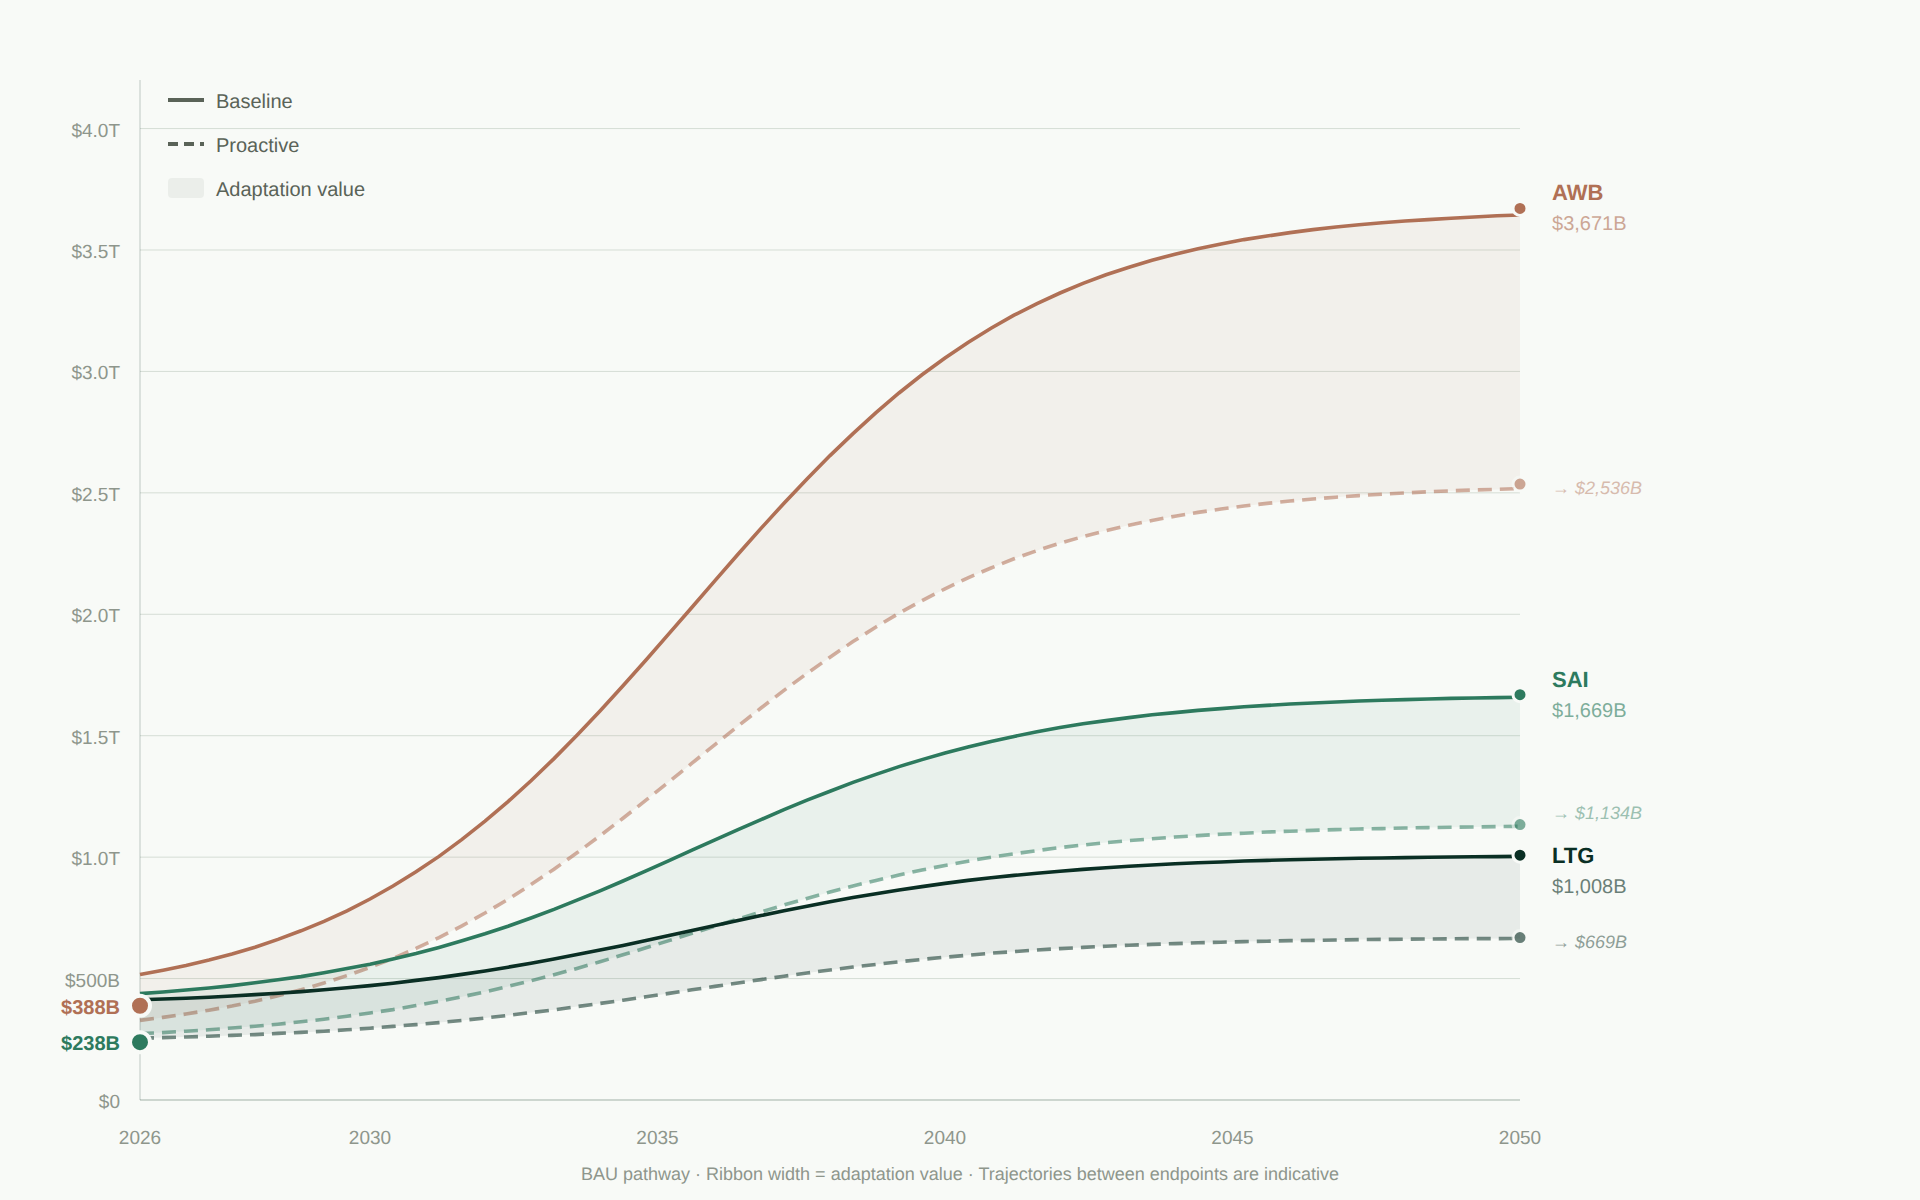
\includegraphics[width=1\textwidth]{images/exhibit22_ribbons.png}
\end{center}
\exhibitsource{Baseline (solid) vs. Proactive adaptation (dashed) under three AI growth scenarios: Limits to Growth, Sustainable AI, Abundance Without Boundaries. Values cumulative over asset lifetimes.}

\begin{pullquote}
The AI build-out does not replicate the installed base's risk profile---it inverts it. Net-zero commitments address 28\% of the exposure on legacy assets but less than 7\% on AI infrastructure. Physical resilience, not energy sourcing, is the binding constraint.
\end{pullquote}

\begin{twocolbody}

{\color{SEGreen}\textbf{A single starting point, three diverging futures}}

\vspace{1mm}

\noindent Exhibit~17 shows how the combined portfolio evolves once AI growth is layered on top of the installed base. All scenarios start from US\$388B of ClimVaR on 90.8~GW and diverge sharply by 2050: about US\$1.0~trillion under Limits to Growth, US\$1.7~trillion under Sustainable AI, and US\$3.7~trillion under Abundance Without Boundaries, with proactive adaptation bending each curve downwards by hundreds of billions.

Two features matter. The curves are convex: most of the increase in ClimVaR occurs between 2030 and 2045, when AI capacity scales fastest. And as scenarios become more aggressive, the gap between Baseline and Proactive widens: in Abundance Without Boundaries, proactive measures avoid over US\$1.1~trillion of cumulative ClimVaR by 2050, yet about US\$2.5~trillion of residual exposure remains, underscoring that adaptation cannot restore a pre-AI risk profile.

A second message is methodological. The \(\times 2.6\) amplification factor mixes physical amplification (higher power density, more climate-exposed sites, concentrated supply chains) and a pure valuation effect (US\$28--42M per MW versus US\$9M for the installed base). The Net Zero Transition pathway illustrates the stakes: carbon costs on the installed base multiply by 6.2, raising total ClimVaR from US\$388B (BAU) to US\$845B (NZT, 83\%), so transition-only strategies (PPAs, grid decarbonization, Scope~2 reduction) can increase total exposure if not paired with physical resilience. Finding~4 shows how a channel-by-channel, region-by-region adaptation portfolio reshapes these trajectories and where the limits of that reshaping lie.

\end{twocolbody}

% ==============================================================================
% FINDING 4 — PAGE 1 of 3
% Portfolio-level adaptation value
% ==============================================================================
% FINDING 4 — PAGE 1 of 2
% ==============================================================================

\clearpage\thispagestyle{chapterstart}

\subsection*{Finding 4: The Adaptation Dividend}
\sectionsubtitle{Adaptation always pays: net exposure falls by 30--39\%}
\greensep

\begin{twocolbody}

\noindent The first three findings quantify a problem; this fourth measures what happens when operators act. Three strategies are compared: \textbf{Baseline} (no climate investment), \textbf{Selective} (one champion action per channel on new builds), and \textbf{Proactive} (systematic adaptation across all assets). All figures are net of adaptation cost.

\end{twocolbody}

\vspace{2mm}
\exhibitcaption{18}{Adaptation value creation---installed base, BAU/MEAN pathway.}
\begin{center}
\datatablesetup
\begin{tabularx}{\textwidth}{l >{\raggedleft\arraybackslash}X >{\raggedleft\arraybackslash}X >{\raggedleft\arraybackslash}X >{\raggedleft\arraybackslash}X >{\raggedleft\arraybackslash}X >{\raggedleft\arraybackslash}X}
\toprule
\datatableheader
\thd{Region} & \thd{CV Baseline} & \thd{CV Selective} & \thd{$\Delta$ Sel.} & \thd{CV Proactive} & \thd{$\Delta$ Proact.} & \thd{Reduction} \\
\midrule
US     & 108 &  89 & 19 &  72 & 36 & 34\% \\
Europe & 107 &  81 & 26 &  60 & 46 & 43\% \\
APMEA  &  62 &  49 & 13 &  39 & 23 & 37\% \\
China  & 111 &  86 & 24 &  67 & 44 & 40\% \\
\midrule
\textbf{Global} & \textbf{388} & \textbf{305} & \textbf{83} & \textbf{238} & \textbf{150} & \textbf{39\%} \\
\bottomrule
\end{tabularx}
\datatableclear
\end{center}

\vspace{2mm}
\exhibitcaption{19}{The adaptation effect: US\$150 billion in net protected value, channel by channel.}
\begin{center}
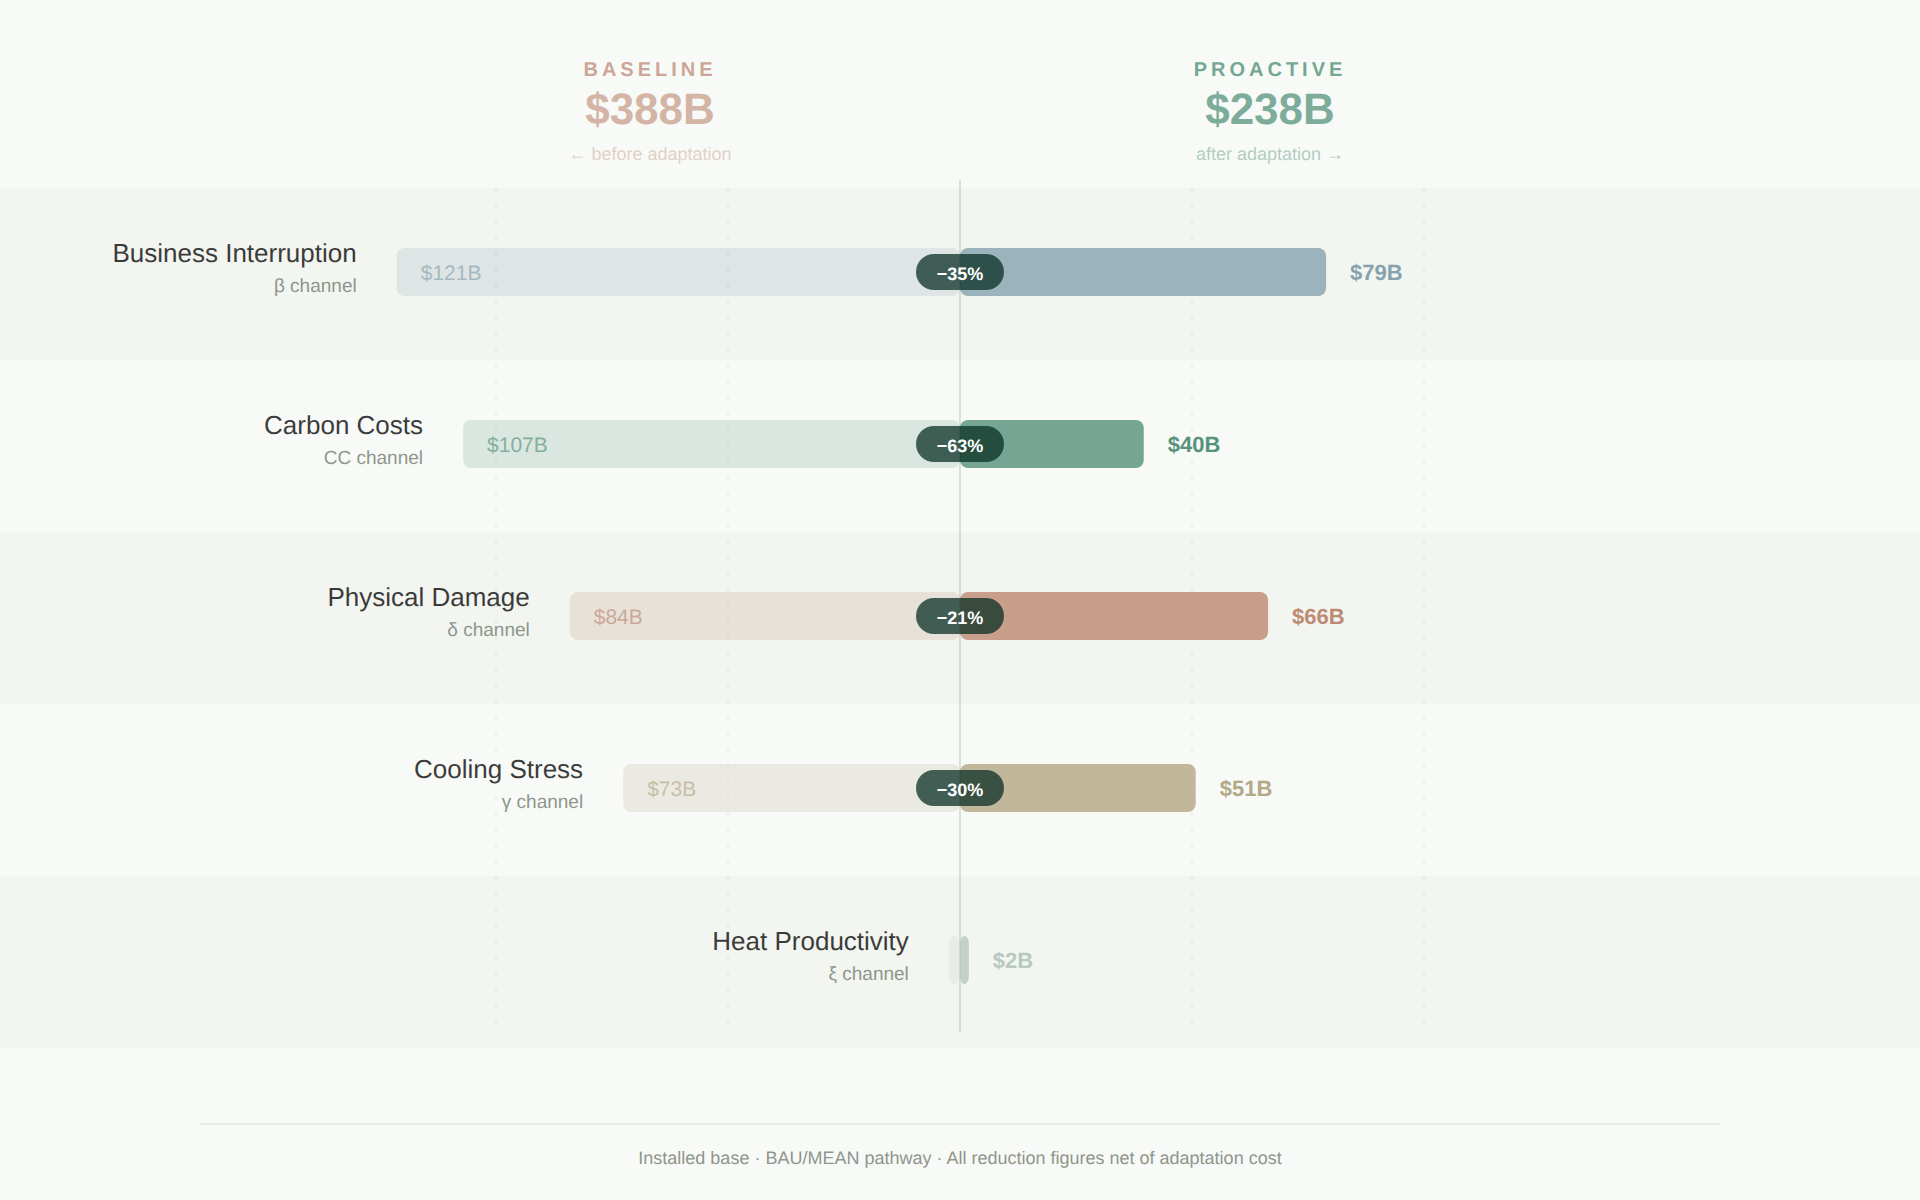
\includegraphics[width=\textwidth]{images/exhibit17_butterfly.png}
\end{center}
\exhibitsource{Left = Baseline; right = Proactive residual. Central badges = net reduction. BAU/MEAN, installed base.}

\begin{twocolbody}

\noindent Proactive adaptation reduces ClimVaR from US\$388B to US\$238B---39\% globally. Europe benefits most (43\%), driven by carbon channel leverage. Carbon compresses fastest; physical channels dominate the residual. Selective captures 56\% of Proactive's value for 15--20\% of CAPEX---the low-regret floor. Proactive adds legacy retrofits and geographic rebalancing, indispensable for the 60--70\% of capacity operating beyond 2040.

\end{twocolbody}

% ==============================================================================
% FINDING 4 — PAGE 2 of 2
% ==============================================================================

\vspace{4mm}
\exhibitcaption{20}{Channel-by-channel waterfall from Baseline to Proactive.}
\begin{center}
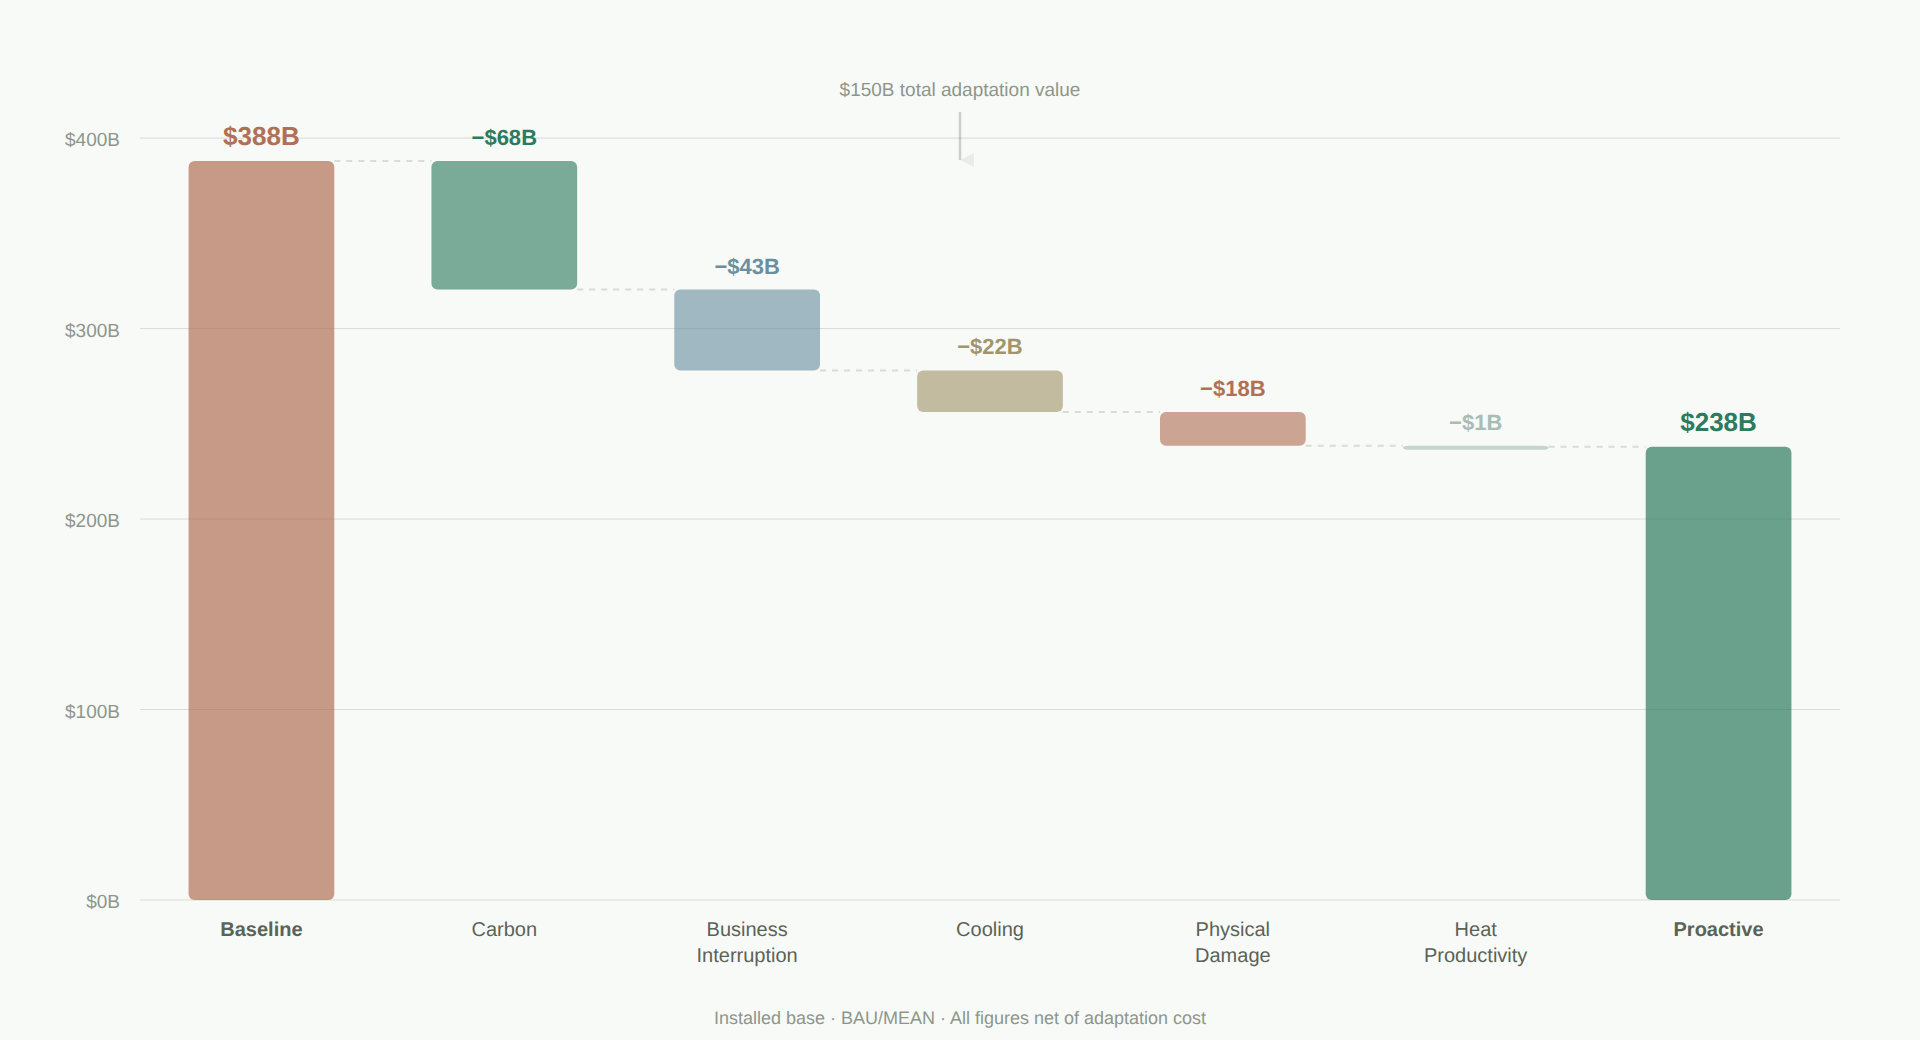
\includegraphics[width=\textwidth]{images/exhibit20_waterfall.png}
\end{center}
\exhibitsource{Each step = one channel's contribution to the US\$150B reduction.}
 
\begin{twocolbody}
 
\noindent Carbon delivers the largest step. Cooling and business interruption follow through liquid cooling, microgrids, and supply chain diversification. Physical damage and heat set the \textit{irreducible floor}: once sited in a floodplain, hardening helps but cannot move the river. Operators who target the tallest steps first live with permanently lower residual risk.
 
\end{twocolbody}
 
\vspace{2mm}
\exhibitcaption{21}{Marginal abatement cost of climate risk: all ten actions below break-even.}
\begin{center}
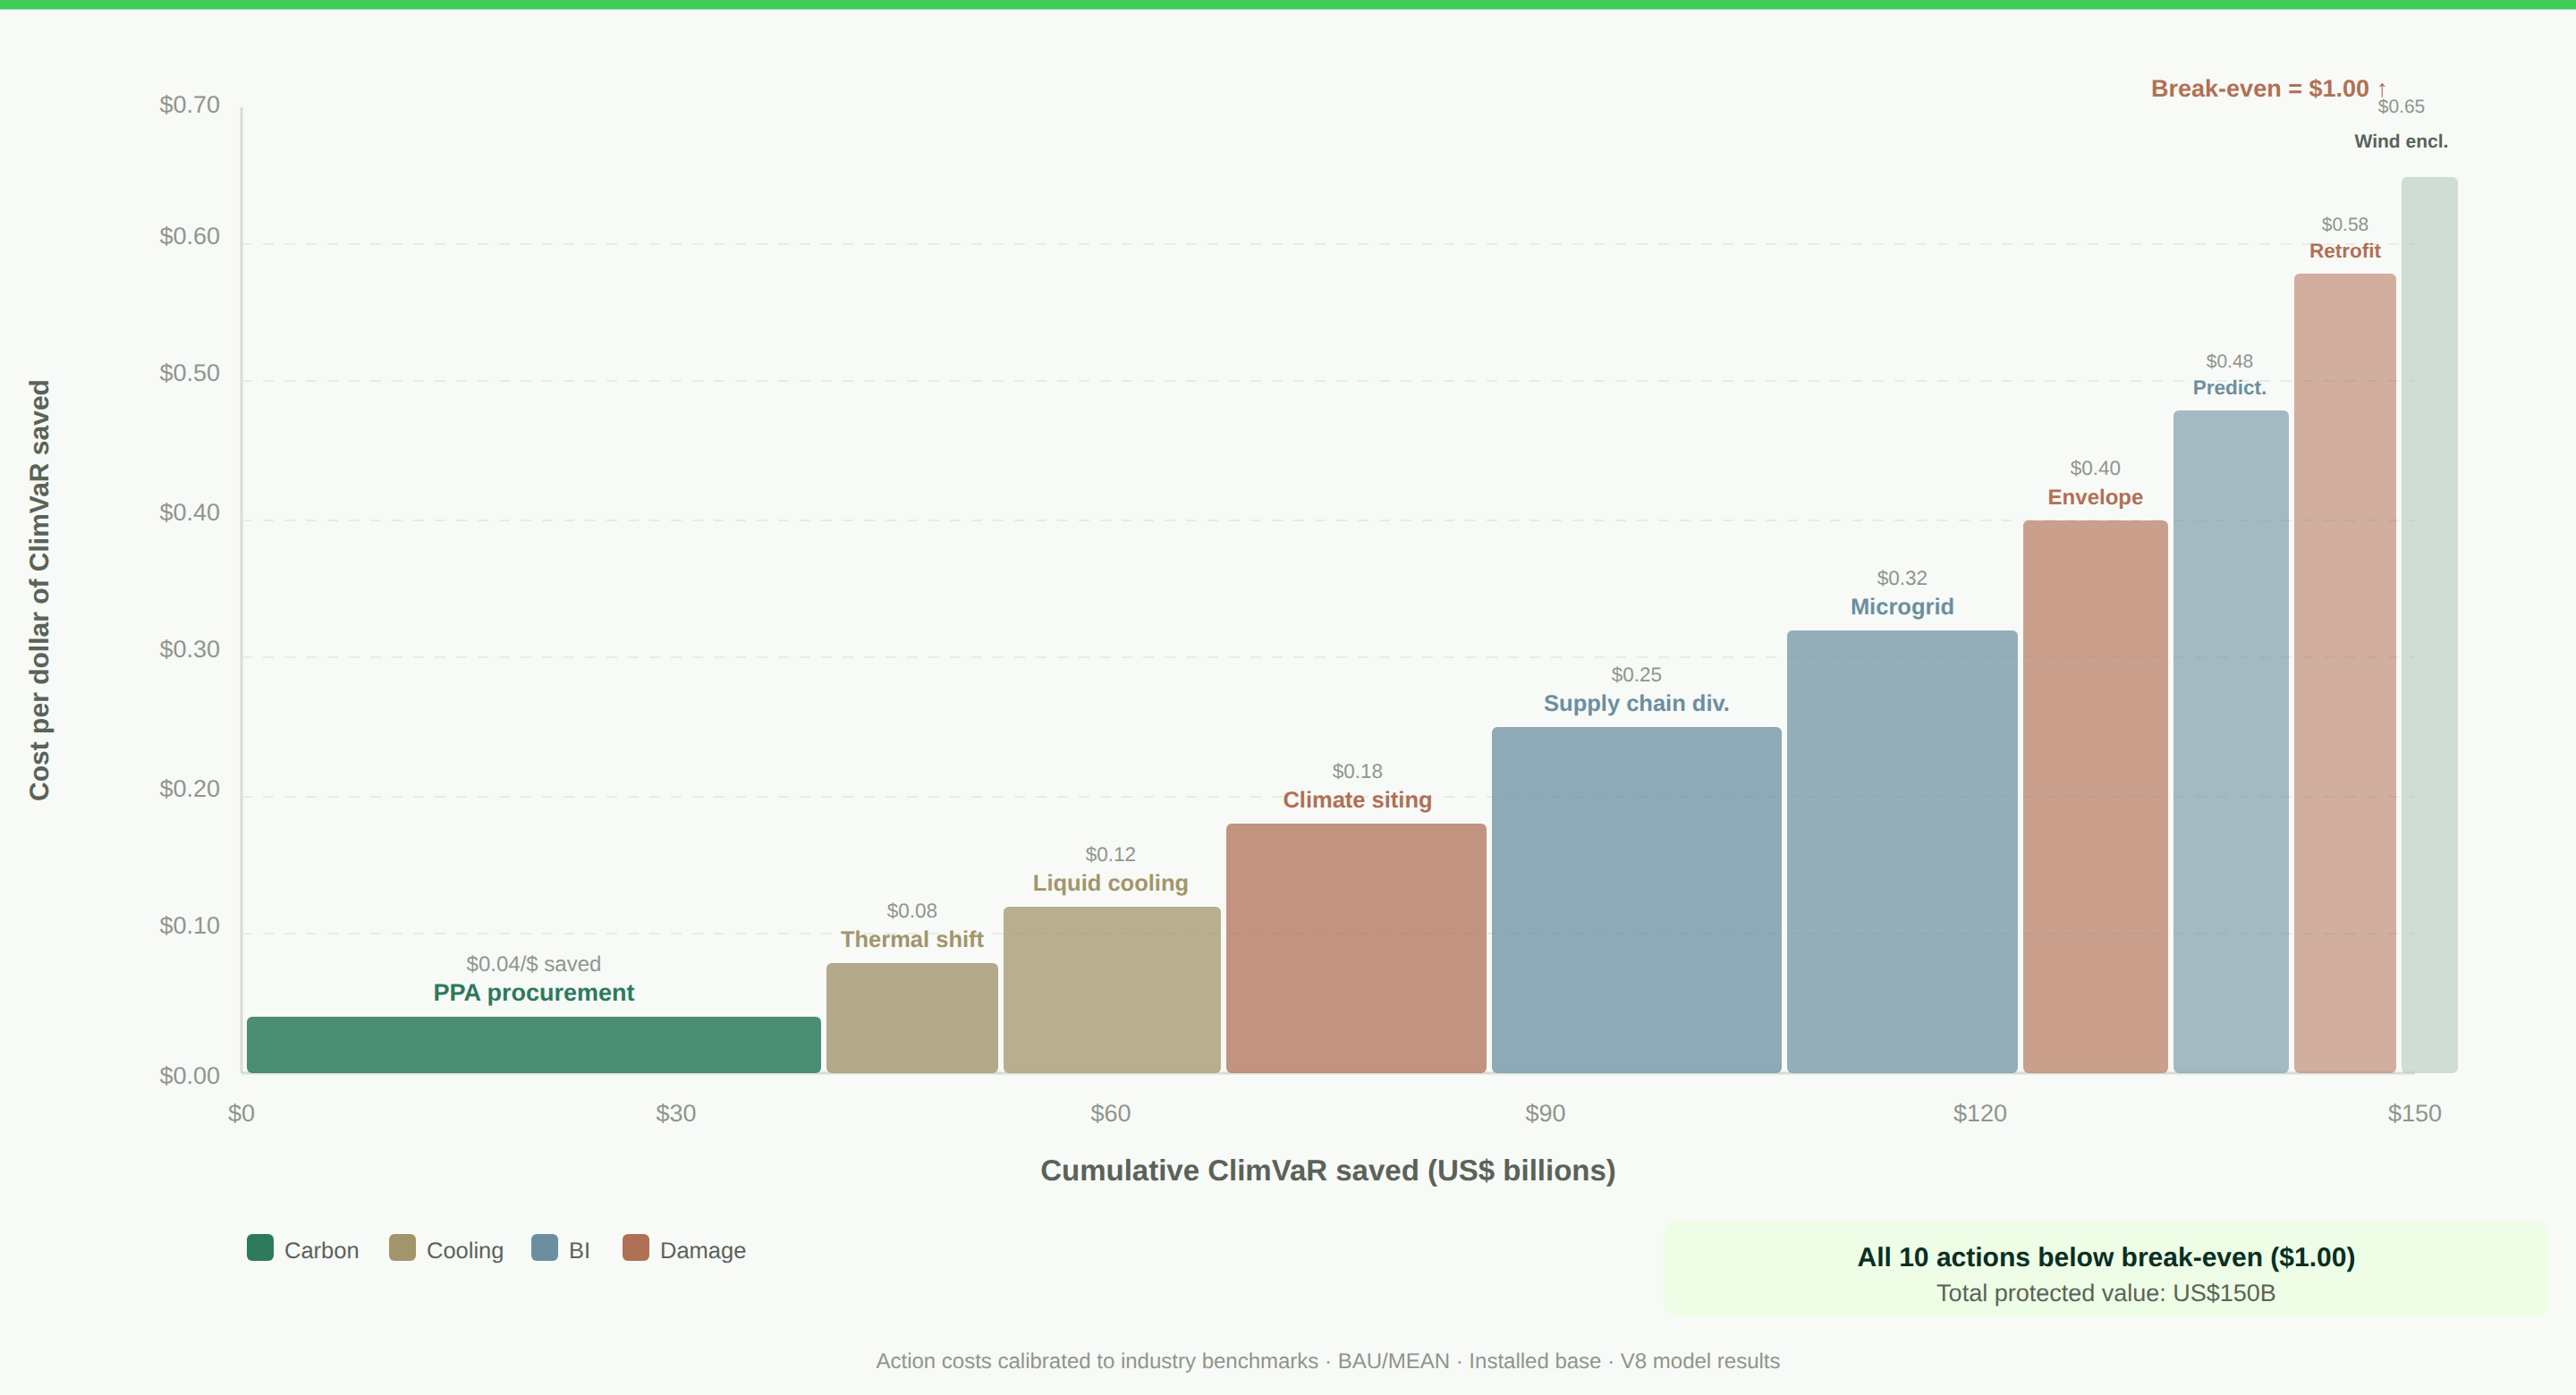
\includegraphics[width=\textwidth]{images/exhibit21_macc.png}
\end{center}
\exhibitsource{All ten actions generate net positive returns. PPAs (US\$0.04/\$ saved), thermal shift, and liquid cooling at design stage are greenfield interventions where resilience is designed in, not retrofitted. The most expensive lever still costs US\$0.65 per dollar of ClimVaR reduced---well below break-even. Action costs calibrated to industry benchmarks.}

% ==============================================================================
% FINDING 4 — PAGE 3: SYNTHESIS — FROM DIAGNOSIS TO STRATEGY
% ==============================================================================

\clearpage\thispagestyle{chapterstart}

\subsection*{Finding 4: The Adaptation Dividend}
\sectionsubtitle{From diagnosis to strategy: scenario sensitivity and the logic of proactive action}
\greensep

\begin{twocolbody}

{\color{SEGreen}\textbf{What the four findings say together}}

\vspace{1mm}

\noindent Read in sequence, the four findings form a single argument. Finding~1 establishes that US\$388~billion of enterprise value is currently unpriced. Finding~2 shows that this exposure varies by a factor of two across regions and, more consequentially, that it differs in composition---so that a dollar of adaptation does not buy the same protection everywhere. Finding~3 demonstrates that AI infrastructure amplifies physical risk by a factor of 2.6 per GW while shifting the portfolio from carbon-dominated to physically-dominated exposure. Finding~4 closes the loop: proactive adaptation reduces installed-base ClimVaR by 39\%, and every one of the ten measured interventions creates net value.

The question is no longer whether climate risk is material for data center portfolios. It is how fast operators convert diagnosis into capital allocation.

\vspace{5mm}

{\color{SEGreen}\textbf{Adaptation as a real option on Net Zero}}

\vspace{1mm}

\noindent The value of adaptation is not fixed; it increases with climate policy ambition. Under the BAU pathway, Proactive adaptation reduces installed-base ClimVaR by about 39\%. Under Net Zero Transition, the same set of actions cuts exposure by more than 50\%, because the carbon channel---where PPAs and energy efficiency are most effective---accounts for a larger share of total risk when carbon prices rise. An operator who signs a long-term PPA in 2026 is not predicting a specific carbon price in 2040. That operator is purchasing upside in high-ambition worlds while still earning positive returns if policy remains weaker and prices stay lower.

This asymmetry gives adaptation the payoff structure of a real option. The cost is paid once, at current prices; the benefit scales with the stringency of future regulation. In a world where the direction of climate policy is clear but the speed is not, this convexity is worth more than a point forecast.

\vspace{5mm}

{\color{SEGreen}\textbf{Matching strategy to portfolio: Selective versus Proactive}}

\vspace{1mm}

\noindent The choice between Selective and Proactive depends primarily on portfolio composition and transition speed. For hyperscalers building mostly new capacity, Selective captures the majority of the adaptation dividend because it targets greenfield assets where marginal cost is lowest and design choices are still reversible. Selective achieves 56\% of Proactive's total risk reduction for 15 to 20\% of capital expenditure---the low-regret floor.

For colocation providers and enterprise operators with large installed bases, Proactive is required to address the 60 to 70\% of capacity that Selective leaves untouched and that will still be operating into the 2040s. Every year of delay converts a greenfield opportunity---where resilience is a line in the design brief---into a future retrofit where it becomes a construction project with higher cost, more downtime, and narrower technical options. The marginal cost curve confirms that even retrofit actions remain below break-even, but the gap between designing in and bolting on is the gap between US\$0.04 and US\$0.65 per dollar of risk saved. Timing is not a secondary consideration; it is the primary determinant of adaptation economics.

\end{twocolbody}

\begin{pullquote}
All ten adaptation levers create net value. The cheapest resilience is designed in, not retrofitted. Every year of delay narrows the technical options and raises the cost per dollar of risk reduced.
\end{pullquote}
 
% CASE STUDIES
% ==============================================================================
\clearpage\thispagestyle{chapterstart}

\subsection*{Three Facility Case Studies}
\sectionsubtitle{Translating aggregate patterns into site-level decisions}
\greensep

\begin{twocolbody}

\noindent Three prospective AI data centers produce ClimVaR intensities ranging from 37.6\% to 167\%, a 4.5$\times$ dispersion at site level. The Shapley decomposition and Leontief analysis produce their most concrete results at this scale. Site~A (US) and Site~B (France) are representative facilities; Site~C (Southern China) is a representative 100~MW allocation reflecting projected AI deployment in the region---its results are indicative of the regional risk profile rather than a specific site assessment.

\end{twocolbody}

\vspace{2mm}
\exhibitcaption{22}{Three prospective AI facilities: site characteristics and ClimVaR decomposition (BAU/MEAN).}

\begin{center}
\datatablesetup
\begin{tabularx}{\textwidth}{>{\raggedright\arraybackslash}p{3.5cm} >{\centering\arraybackslash}X >{\centering\arraybackslash}X >{\centering\arraybackslash}X}
\toprule
\datatableheader
& \thd{Site~A (US South)} & \thd{Site~B (France)} & \thd{Site~C (S.~China)} \\
\midrule
Operator / Project        & Major AI hyperscaler      & Sovereign AI project & Major coastal delta \\
Capacity                  & 2,800~MW            & 100~MW             & 100~MW \\
Enterprise value (V$_0$)  & \$1.9B              & \$2.1B             & \$1.4B \\
PUE                       & 1.15                & 1.12               & 1.28 \\
\midrule
Business interruption     & \$384M (43\%)       & \$374M (11\%)      & \$276M (53\%) \\
Cooling                   & \$336M (37\%)       & \$459M (13\%)      & \$96M (18\%)  \\
Physical damage           & \$143M (16\%)       & \$2,678M (75\%)    & \$29M (6\%)   \\
Carbon                    & \$28M (3\%)         & \$42M (1\%)        & \$113M (22\%) \\
Heat productivity         & \$11M (1\%)         & \$6M ($<$1\%)      & \$4M (1\%)    \\
\midrule
\textbf{Total ClimVaR}    & \textbf{\$902M}     & \textbf{\$3,560M}  & \textbf{\$517M} \\
\textbf{Intensity}        & \textbf{46.5\%}     & \textbf{167\%}     & \textbf{37.6\%} \\
\bottomrule
\end{tabularx}
\datatableclear
\end{center}

\exhibitsource{V8 model results. BI includes direct + supply chain (Leontief). Enterprise values at facility level. Site~C is a probabilistic allocation; results are indicative before site-specific due diligence. The same table structure can be replicated for any facility once site-level financial, hazard, and engineering data are available.}

\begin{twocolbody}

\subsubsection*{Site~A (US) — The Supply Chain Problem}

\paragraph{A moderate intensity with hidden drivers.}
The largest announced AI facility in the world carries a moderate 46.5\% ClimVaR intensity, apparently safer than many legacy sites. But business interruption (43\%) and cooling (37\%) dominate the profile, while carbon and heat play only marginal roles. On paper, Site~A looks like a robust, low-carbon, low-damage location.

\paragraph{Risk imported through global supply chains.}
The Shapley decomposition shows that 56\% of Site~A’s business interruption risk comes from tropical wind propagating through semiconductor and power-equipment supply chains. A facility sited in the semi-arid plains of the US South derives more than half its BI exposure from cyclones thousands of kilometers away. Direct on-site hazards account for less than 1\% of BI: Site~A’s risk is not where Site~A is, it is where its suppliers are.

\subsubsection*{Site~B (France) — The Flood Trap}

\paragraph{A “safe” location with 167\% intensity.}
A temperate European site often perceived as safe carries 167\% ClimVaR intensity: its climate-adjusted risk exceeds its entire enterprise value. River flood damage (\$2.7B, 75\% of total) dominates, far ahead of BI, cooling, or carbon. The river valley’s fluvial hazard profile, combined with the site’s proximity to the river, produces an exposure that generic checklists do not flag.

\paragraph{From screening signal to targeted assessment.}
Site~B demonstrates the value of the framework as an early-warning tool: without granular hazard attribution, generic assessments would classify this site as low-risk. The 167\% figure is not a literal forecast; it reflects archetype-based calibration and should be read as a strong screening signal that flood exposure merits detailed engineering assessment. The model identifies the question; the answer requires site-specific data on elevation, flood defenses, building envelope, and drainage design.

\subsubsection*{Site~C (Southern China) — The Triple Threat}

\paragraph{A balanced but complex risk fingerprint.}
Site~C’s 37.6\% intensity looks modest next to Site~B, but the composition is more complex: business interruption (53\%), carbon (22\%), and cooling (18\%) form a three-pronged profile. The region combines typhoon exposure along critical supply chains, high grid carbon intensity, and subtropical heat stress, with each channel contributing a substantial share.

\paragraph{No single silver bullet.}
Site~C is the prototypical case where no single adaptation lever reduces more than a quarter of total exposure. Microgrids can dampen BI, PPAs reduce the carbon wedge, and high-efficiency cooling cuts thermal loads, but none of these alone shifts the site into a low-risk regime. Effective risk reduction requires a \textit{multi-channel} package applied in parallel.

\subsubsection*{From portfolio analytics to site-level decisions}

\paragraph{Re-using the same machinery at finer grain.}
All the analytical machinery developed for the 8,572-facility portfolio can be replicated at individual site level, where more qualitative and engineering data are available. For Site~B, local information on levees, flood defenses, elevation, and building standards can replace archetype assumptions and either confirm or recalibrate the 167\% signal. For Site~A, a detailed supply chain audit can refine Leontief coefficients, distinguishing between easily substitutable components and true single points of failure.

\paragraph{A consistent framework across scales.}
The framework is deliberately designed to operate at both scales without modification: the same ClimVaR, Shapley, and Leontief structures that aggregate risk across regions can be “zoomed in” to support investment committees, permitting decisions, and asset-level adaptation roadmaps. The case studies show how aggregate findings translate into concrete site-level questions: \textit{which channel dominates, which hazards drive it, and which interventions change the answer fastest?}

\end{twocolbody}

\vspace{2mm}
\exhibitcaption{23}{Hazard attribution (Shapley) and propagation pathway (Leontief) at three sites.}

\begin{center}
\datatablesetup
\begin{tabularx}{\textwidth}{>{\raggedright\arraybackslash}p{3.5cm} >{\centering\arraybackslash}X >{\centering\arraybackslash}X >{\centering\arraybackslash}X}
\toprule
\datatableheader
& \thd{Site~A (US South)} & \thd{Site~B (France)} & \thd{Site~C (S.~China)} \\
\midrule
\multicolumn{4}{l}{\textbf{BI: hazard attribution (Shapley)}} \\
Tropical wind / cyclone & 56\% & 52\% & 60\% \\
Storm (convective)      & 24\% & 22\% & 27\% \\
Drought                 & 15\% & 23\% & 8\%  \\
\midrule
\multicolumn{4}{l}{\textbf{BI: propagation pathway (Leontief)}} \\
Direct operations       & $<$1\% & 2\%  & 2\%  \\
Supply chain (indirect) & $>$99\% & 98\% & 98\% \\
\midrule
\multicolumn{4}{l}{\textbf{Damage: dominant hazard}} \\
                        & Fire (97\%) & River flood (100\%) & Fire (79\%) \\
\bottomrule
\end{tabularx}
\datatableclear
\end{center}

\exhibitsource{Shapley: 32 coalitions per facility. Leontief: OECD MRIOT 2023.}

\exhibitcaption{24}{Three sites, three risk profiles: channel decomposition at facility level.}
\begin{center}
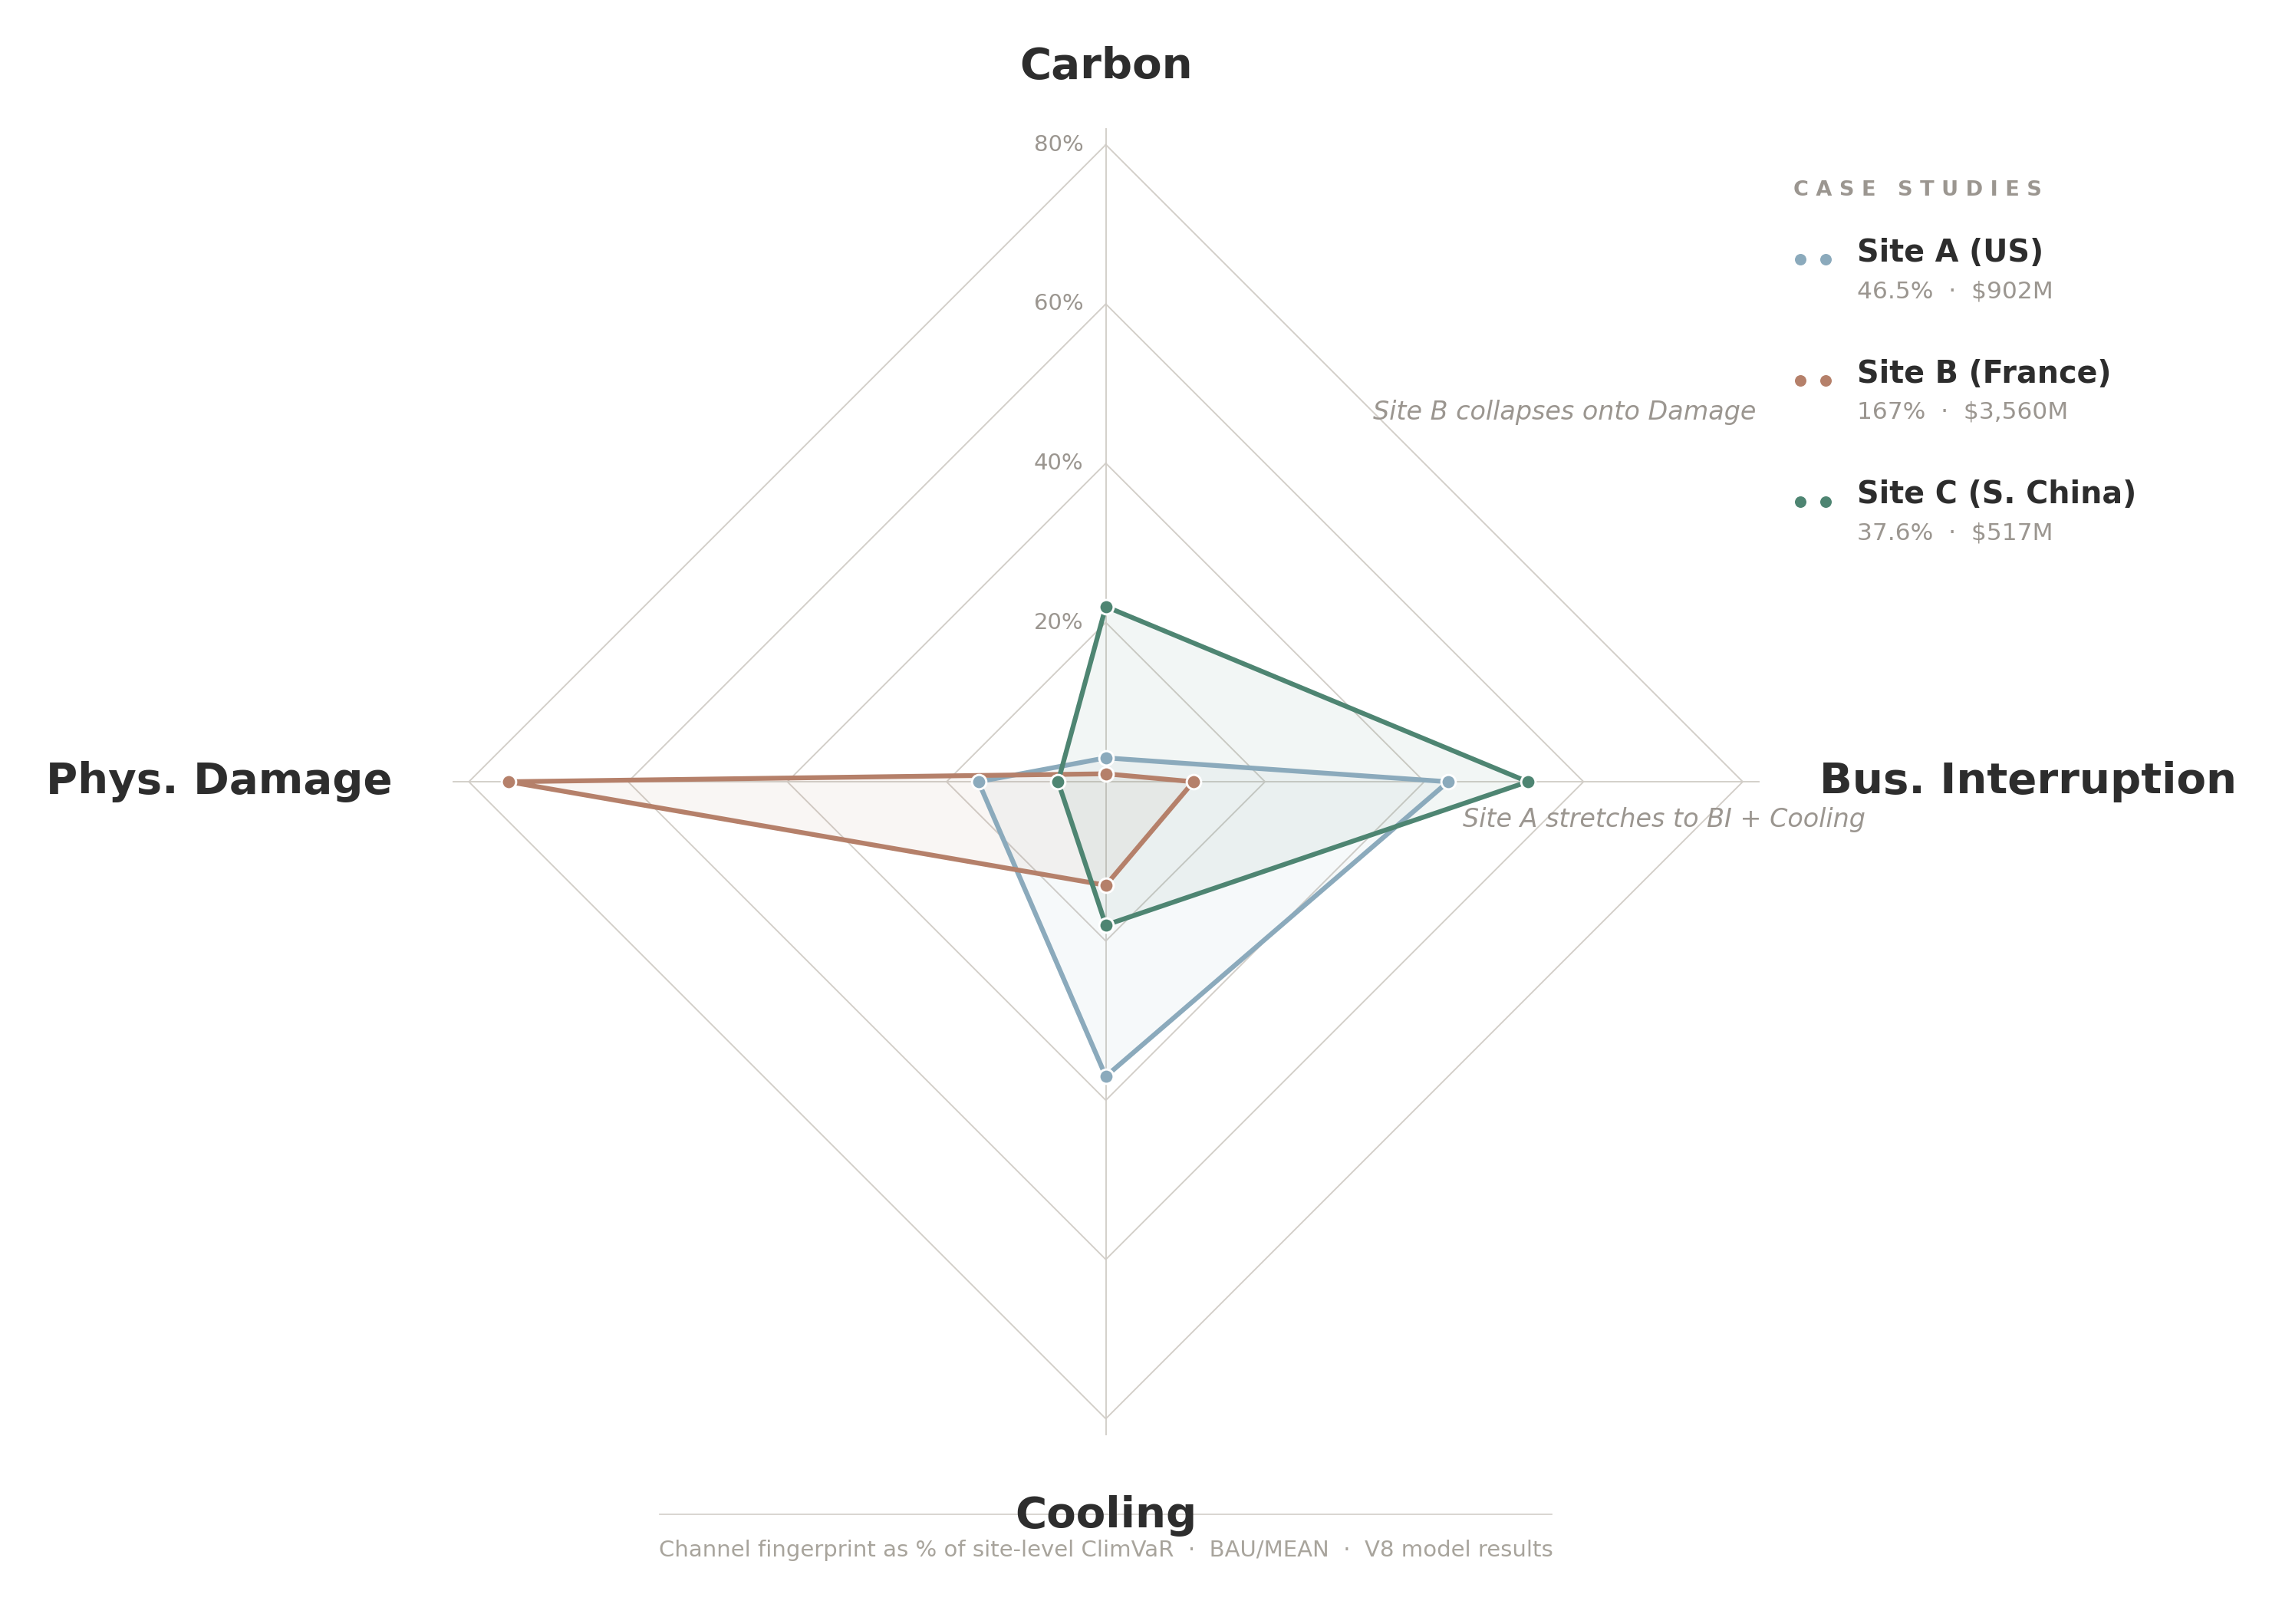
\includegraphics[width=0.90\textwidth]{images/exhibit22_triptych.png}
\end{center}
\exhibitsource{Radar overlay: each polygon is one facility's channel fingerprint (\% of site-level ClimVaR). Site~A stretches toward BI and Cooling; Site~B collapses onto Damage; Site~C is balanced. Overlaying profiles makes the contrast between risk architectures immediately visible.}

% Advisory Services box moved to standalone page after Chapter IV — see advisory-box.tex

% ==============================================================================
% DISCUSSION
% ==============================================================================
\clearpage\thispagestyle{chapterstart}

\subsection*{Discussion}
\sectionsubtitle{Interpretation and systemic implications}
\greensep

\begin{twocolbody}

\subsubsection*{The \$388 Billion Baseline in Context}

\noindent The US\$388~billion ClimVaR on the installed base (38.3\% of enterprise value) can be situated against three reference points. The WEF/S\&P aggregate of US\$3.3~trillion by 2055 operates at a different analytical level, but the order of magnitude is consistent when discounting and scope differences are accounted for \citep{wef2025}. XDI covers comparable facility counts but reports structural damage metrics rather than enterprise value loss; our framework extends this by adding cooling stress, carbon pricing, and supply chain propagation---channels that account for 65--75\% of total ClimVaR \citep{xdi2025}. Dietz et al.\ (2016) estimated 1.8\% of global financial assets at risk; the 38\% intensity for data centers reflects the sector's higher exposure through energy costs, uptime requirements, and supply chain concentration.

The \$388B figure represents a lower bound on total economic exposure. The framework quantifies private financial risk but does not capture systemic externalities: grid strain from concentrated AI load, water resource competition between data centers and agriculture, community displacement from extreme events, or the cascading economic effects of simultaneous service interruptions across interconnected facilities. These excluded channels would increase, not decrease, the total.

The gap between 38\% enterprise value erosion and zero in standard DCF valuations quantifies the mispricing. Concurrent work in portfolio management confirms this gap from the asset allocation side: \citet{luciani2026} show that physical climate risk lacks the standardized anchor metric equivalent to carbon intensity, and that reducing portfolio-level physical exposure beyond 10\% destabilizes diversified portfolios---the facility-level ClimVaR framework developed here is designed to provide this missing metric.

\subsubsection*{The Supply Chain Multiplier}

The $\times$11 ratio of supply chain to direct business interruption is the most consequential finding for risk management practice. At all three case study sites, 98--99\% of business interruption propagates through supply chains rather than from direct on-site hazards. Taiwan accounts for over 60\% of advanced semiconductor fabrication; large power transformers carry 12--24 month lead times; high-bandwidth memory production concentrates in South Korea. A single typhoon disrupting TSMC operations would propagate through every data center in the global portfolio via the Leontief inverse \citep{verdantix2024}.

The Leontief framework assumes fixed technical coefficients---firms cannot reroute sourcing under stress. Long-duration disruptions are partially attenuated by adaptive behavior not captured in the model. The $\times$11 multiplier is an upper bound for prolonged disruptions and a reasonable estimate for acute shocks. More fundamentally, the approach relies on aggregate multi-regional input-output tables rather than on the actual supply chain of each facility. Where facility-specific procurement data are available---bills of materials, qualified vendor lists, logistics routing---they should replace the MRIOT coefficients, yielding sharper estimates of both the multiplier and its geographic decomposition. The present results establish the order of magnitude and the direction; facility-level supply chain audits are the natural next step.

\subsubsection*{Physical Risk is Systemic}

The residual 61\% of ClimVaR that proactive adaptation cannot eliminate is not a failure of the framework---it reflects a structural reality. \citet{luciani2026} reach an analogous conclusion from the portfolio management side: ``physical risk is largely systemic, and systemic risks are difficult---if not impossible---to diversify.'' Their analysis shows that constraining physical risk exposure by even 10\% reduces investable portfolios to fewer than 200 stocks, with tracking error volatility rising by an order of magnitude compared to equivalent carbon constraints. Our facility-level results and their portfolio-level results converge on the same conclusion: the fraction of physical climate risk that individual actors can manage is bounded, and the remainder requires collective instruments---public risk-sharing, infrastructure stress tests, and regulatory frameworks calibrated to actual financial exposure.

\end{twocolbody}